\documentclass{beamer}
\usepackage{graphicx}
\usepackage{subfigure}
\usepackage{amsmath,amssymb,amsthm}
\usepackage{mathtools}
\usepackage{epsfig}
\usepackage{color,soul}
\usepackage{geometry}
\usepackage{hyperref}
\usepackage{lmodern}
\usepackage{wrapfig}
\usepackage[backend=biber]{biblatex}
\theoremstyle{plain}
\newtheorem{thm}{Theorem}[section]
\theoremstyle{definition}
\newtheorem{exm}[thm]{Example}
\newtheorem{defi}[thm]{Definition}
\newtheorem{lemm}[thm]{Lemma}
\newtheorem{conj}[thm]{Conjecture}
\newtheorem{cond}[thm]{Condition}
\newtheorem{cor}[thm]{Corollary}
\usetheme{Rochester}

\graphicspath{ {Figures/} }

\addbibresource{ETcell.bib}

\title{Multi-element probabilistic collocation method for sensitivity analysis}
\author{Ryan Viertel}
\institute{University of Utah}
\date{Nov. 21, 2016}

\begin{document}

\begin{frame}
\titlepage
\end{frame}

\begin{frame}
\frametitle{Table of Contents}
\tableofcontents
\end{frame}

\AtBeginSection[]
{
    \begin{frame}
    \frametitle{Outline}
    \tableofcontents[currentsection]
    \end{frame}
}

\section{Introduction}

\begin{frame}\frametitle{CES Masters Project}
  This work represents the final project for my MS degree in Computational Engineering and Science.
\newline
\newline
  Goals of the project:
  \begin{itemize}
    \item Build an efficient implementation of the ME-PCM method% for sensitivity analysis. This method should be written in parallel and allow investigation of an arbitrary finite dimensional parameter space for an arbitrary system of ODEs.
    \item Analyze Stability of ET-Cell Model
    \item Run this implementation on University of Utah CHPC clusters% to allow for more data collection than would be possible on a personal computer or though math department resources.
    \item Analyze the collected data to make new conclusion about the stability and behavior of the ET cell.
  \end{itemize}
\end{frame}

\begin{frame}\frametitle{ME-PCM Introduction}
\begin{itemize}
  \item The ME-PCM is described in the paper \emph{Multi-element probabilistic collocation method for sensitivity analysis in cellular signaling networks} \cite{foo_multi-element_2009}
  \item An alternative to monte-carlo simulations and gradient-based methods for analyzing ODE or PDE system sensitivity.
  \item Has the advantages that:
    \begin{itemize}
     \item It is more computationally efficient
     \item Can provide a comparison of various output metrics of the system with minimal added computational cost
     \item Output metrics can be functions of time to allow for sensitivity analysis of a transient response
     \item Utilizes numerical quadrature principles
    \end{itemize}
  \item Can help elucidate and quantify the effects of system parameters
\end{itemize}
\end{frame}

\section{ET-Cell Model}

\begin{frame}\frametitle{Diagram of Olfactory Bulb}
  \begin{center}
   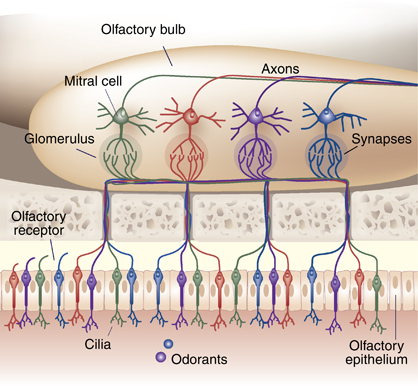
\includegraphics[scale = .8]{glomerularLayer.jpg}
  \end{center}
  nature.com
\end{frame}

\begin{frame}\frametitle{Glomerulus}
  \begin{center}
   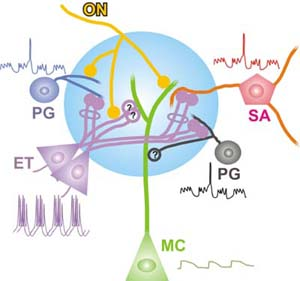
\includegraphics[scale = 2.6]{glomerulus.jpg}
  \end{center}
  http://www.uams.edu/ctn/research/hayar.asp
\end{frame}

\begin{frame}\frametitle{ET Cell Bursting}
 \begin{itemize}
  \item Each ET cell has a bursting frequency in the range of .2 - 10 Hz
  \item Bursting is intrinsic to the cell, and continues even after blocking synaptic activity
  \item Bursts ride on a slow depolarizing envelope
  \item Conceptual model of the ET cell is proposed in Liu \& Shiply 2008 \cite{liu_multiple_2008}
 \end{itemize}
 \begin{center}
  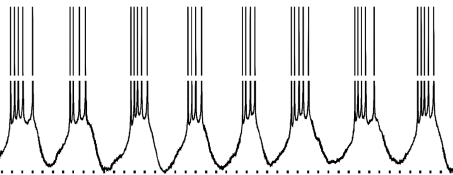
\includegraphics[scale = .4]{trace.png}
 \end{center}
 fig. 1 G
\end{frame}

\begin{frame}\frametitle{Summary of Experimental Results from Liu \& Shipley \cite{liu_multiple_2008}}
  \begin{center}
    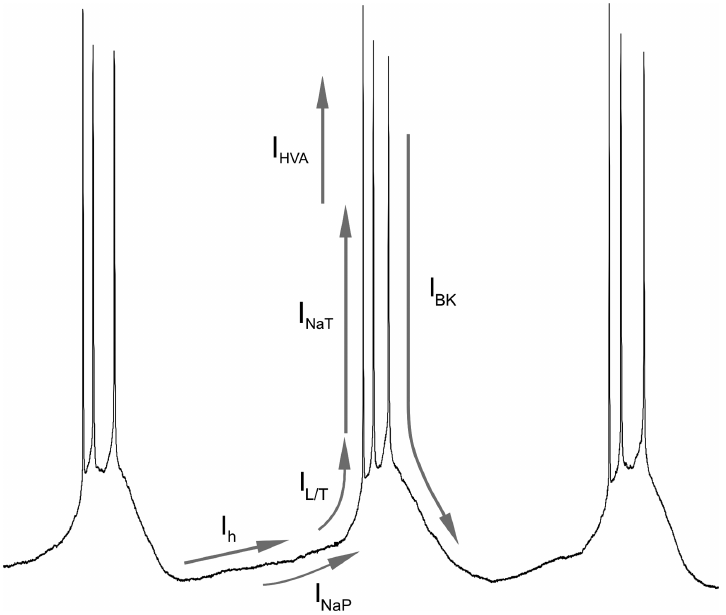
\includegraphics[scale = .33]{summary.png}
  \end{center}
\end{frame}

 \begin{frame}\frametitle{Model}
 We track the membrane potential, the calcium concentration, and the state of the gating variables for each current.
 \begin{align*}
   C\frac{dV}{dt} &= -(I_h + I_{NaP} + I_{LVA} + I_{Na^+} + I_k + I_{HVA} + I_{BK} + I_{new} + I_{app})\\[1em]
   I_x &= g_xm_x^ph_x^q(V - V_x)\\[1em]
   \frac{d[Ca]}{dt} &= -\gamma\frac{I_{LVA} + I_{HVA}}{zFd} + \frac{[Ca_0] - [Ca]}{\tau_{Ca}}
 \end{align*}
 \end{frame}

 % \begin{frame}\frametitle{Gating variables}
 % Each gating variable has the form
 % $$\frac{dw}{dt} = (w_{\infty}(V) - w)/\tau_{w}(V)$$
 % Where $w_{\infty}$ and $\tau_{w}$ depend on $V$.\\
 % \vspace{1em}
 % In the case of the $BK$ current, also depends on $[Ca^{2+}]$
 % $$w_{\infty} = \frac{1}{1 + \exp{(V_{1/2} - V)/15.6}}$$
 % $$V_{1/2} = -20 + 59.2e^{-90[Ca]} + 96.7e^{-470[Ca]}$$
 % \end{frame}

 \begin{frame}\frametitle{Computational Model}
   \begin{center}
     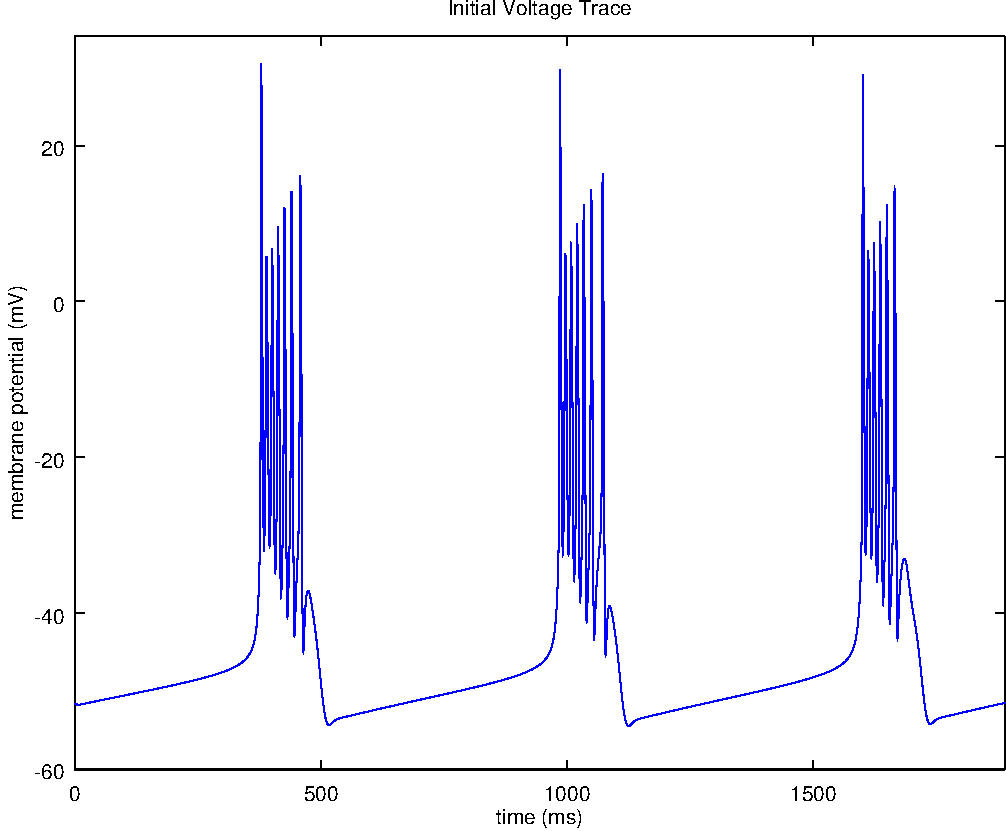
\includegraphics[scale = .5]{initialTrace.pdf}
   \end{center}
 \end{frame}

 \section{Method}

 \begin{frame}\frametitle{ME-PCM Method}
   We will consider a generic system of ODEs
   \begin{equation*}
     \mathbf{x}'(t) = f(\mathbf{x}(t),\mathbf{Y},t)
   \end{equation*}
   Where $\mathbf{x}$ is a vector of system variables, and $\mathbf{Y}$ is a vector of parameters or initial conditions that we will vary. We will consider $\mathbf{Y}$ to be stochastic with a uniform distribution on its domain. There are 3 steps to the ME-PCM:
   \begin{enumerate}
     \item Select biologically relevant output metrics of the system
     \item Select a parameter space, split the parameter space up into elements, and define a quadrature rule for integration over each element
     \item Sample solutions over parameter space and compute the metrics of system output
   \end{enumerate}
 \end{frame}

 \begin{frame}\frametitle{ME-PCM Method}
   \begin{center}
     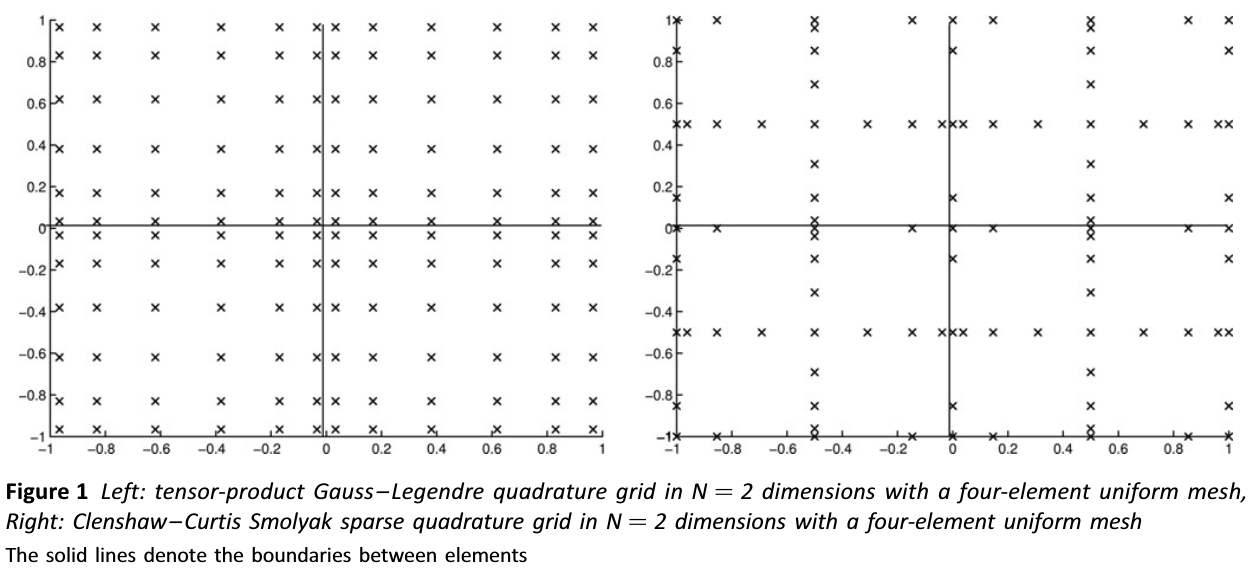
\includegraphics[scale = .25]{grid.png}
   \end{center}
 \end{frame}

 \begin{frame}\frametitle{1. Select statistical metrics for system output}
   Biologically relevant metrics are defined in terms of statistical moments. In our case we chose to measure the mean and variance of the following quantities
   \begin{enumerate}
     \item Burst Duration
     \item Burst Frequency
     \item Spikes Per Burst
     \item Minimum Membrane Potential
     \item Average Membrane Potential
     \item Peak Firing Rate
     \item Average Firing Rate
   \end{enumerate}
 \end{frame}

\begin{frame}\frametitle{2a. Select a parameter space}
  We chose to analyze the relative strengths of the maximum conductance levels for the following currents
 \begin{itemize}
   \item The Hyperpolarization-activated cation current - Ih
   \item Low voltage activated Calcium current - ILVA
   \item Persistent sodium current - INaP
   \item Large conductance potassium current - IBK
 \end{itemize}

 Currents were varied by $\pm$ $30\%$ of their default value
\end{frame}

\begin{frame}\frametitle{2b. Select a quadrature rule}
  Gauss-Legendre Quadrature:
  \begin{itemize}
    \item General, commonly used integration rule
    \item Good at integrating functions that can be well approximated by polynomials
    \item Gives exact answer for polynomials of degree 2n-1 ($n = \#$ of grid points in each direction)
    \item Grid points are locations of the roots of Legendre polynomials $P_n(x)$
    \item Weights are given by:
  \end{itemize}

  \begin{equation*}
    w_i = \frac{2}{(1-x_i^2)(P'(x_i))^2}
  \end{equation*}

\end{frame}

\begin{frame}\frametitle{3. Sample Solutions and Compute Metrics}
  \begin{center}
    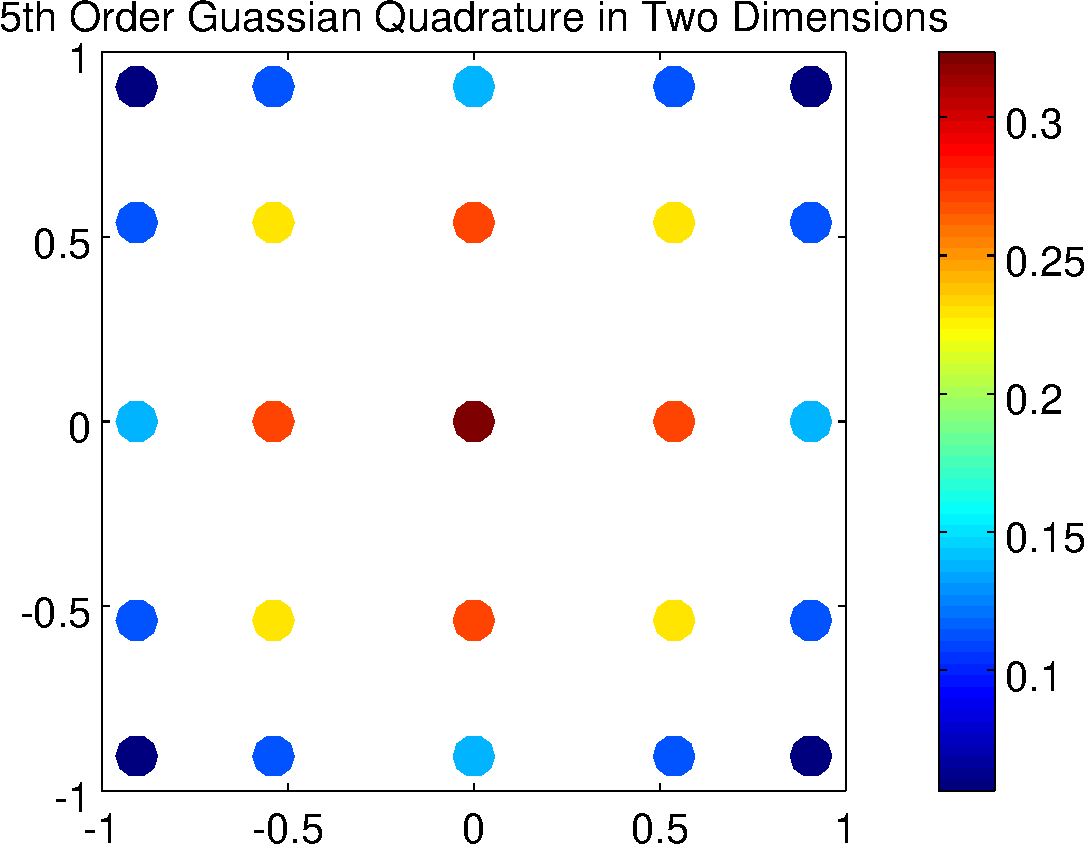
\includegraphics[scale = .5]{gaussian-quadrature.pdf}
  \end{center}
\end{frame}

% \begin{frame}\frametitle{3. Sample solutions and compute metrics}
%  \begin{itemize}
%   \item Compute the solution at each sample point (quadrature point) in the parameter space.
%   \item Compute the value of each metric within a given element by integrating over the parameter space on the grid in that element
%   \item For example, the burst duration sensitivity, $D_k$, in element $E_k$ is given by
%
%   \begin{equation*}
%    \left[\frac{1}{Vol(E_k)}\sum_{i=1}^{625}{D_k^2(x_k^i)w_k^i}\right] - \left[\frac{1}{Vol(E_k)}\sum_{i=1}^{625}{D_k(x_k^i)w_k^i}\right]^2
%   \end{equation*}
%  \end{itemize}
% \end{frame}

\section{Implementation}

\begin{frame}\frametitle{Implementation}
  The code for this project was written in C and is available at \href{https://github.com/rviertel2/CES-project}{https://github.com/rviertel2/CES-project}\\

  \vspace{1em}

  The following open source libraries/APIs were used in this project:
  \begin{itemize}
    \item GSL - GNU Scientific Library (\href{https://www.gnu.org/software/gsl/}{https://www.gnu.org/software/gsl/})
    \item OpenMP - Open Multi-Processing (\href{http://www.openmp.org/}{http://www.openmp.org/})
    \item OpenMPI - A High Performance Message Passing Library (\href{https://www.open-mpi.org/}{https://www.open-mpi.org/})
  \end{itemize}
\end{frame}

\begin{frame}\frametitle{Parallelization}
  \begin{center}
    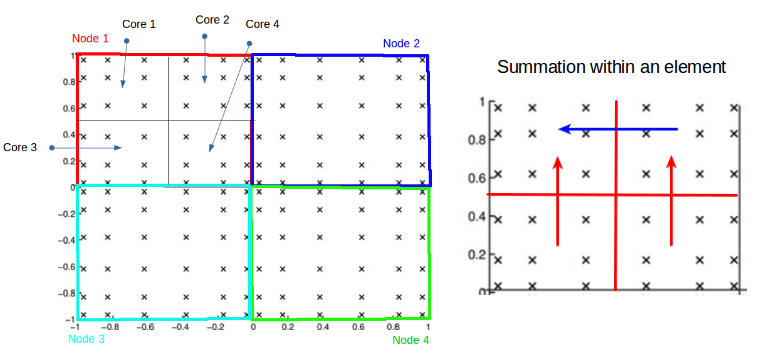
\includegraphics[scale=.42]{parallel.png}%
  \end{center}
\end{frame}

\begin{frame}\frametitle{Parallelization}
  This Hybrid shared/distributed memory approach has the nice properties that:
  \begin{enumerate}
    \item It allows for use of multiple nodes, and complete use of all resources
    \item It avoids any message passing
    \item It naturally fits the hierarchy of elements and grid points
    \item It was more simple to implement than an MPI only or OpenMP only approach
  \end{enumerate}
\end{frame}

\begin{frame}\frametitle{Computation}
  \begin{itemize}
    \item $625$ elements x $625$ grid points $= 390625$ total simulations
    \item Simulations took about 10 seconds each
    \item Total running time in serial $\approx O(1000)$ hours
    \item Run on Ember cluster (CHPC) with 11 Nodes
    \begin{itemize}
      \item Dual Socket-Six core nodes (12 cores per node)
      \item 2.8 GHz Intel Xeon (Westmere X5660) processors
      \item 24 Gigs Memory per Node
    \end{itemize}
    \item Total running time was $\approx 6$ hours 40 min
    \item Linear speed up achieved as expected.
  \end{itemize}
\end{frame}

\begin{frame}\frametitle{Indexing}
  4 dimensional parameter space split up into 5 elements in each direction. $5^4 = 625$ total elements.\\
  \vspace{1em}
  Elements were numbered in counting order

  \begin{center}
    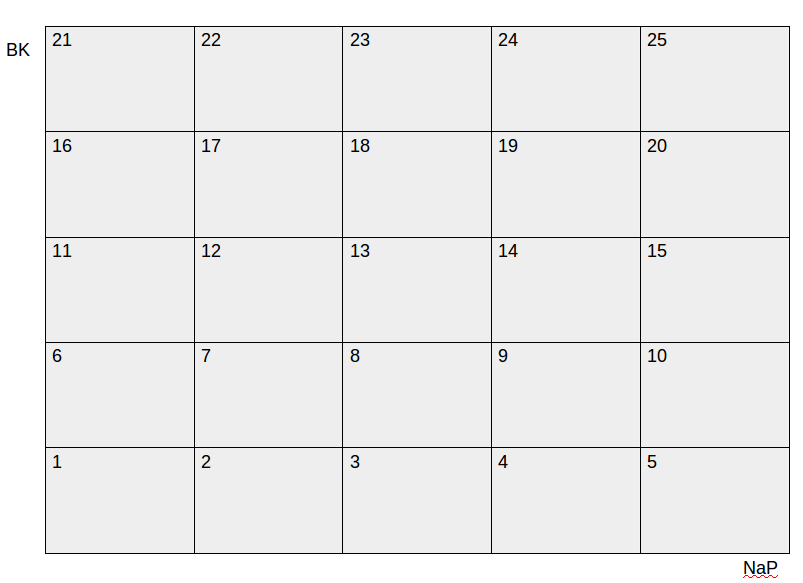
\includegraphics[scale=.25]{indexing.png}%
  \end{center}
\end{frame}

\begin{frame}\frametitle{Indexing}
  \begin{center}
    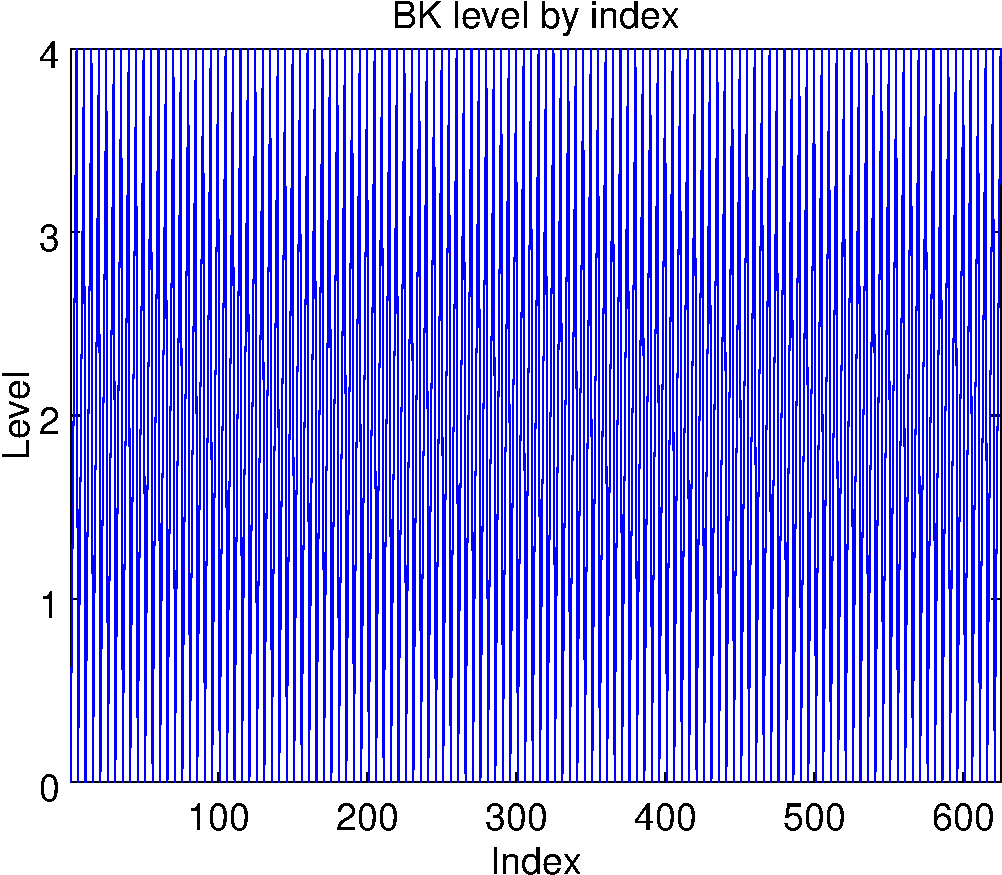
\includegraphics[scale=.32]{BKfrequency.pdf}%
    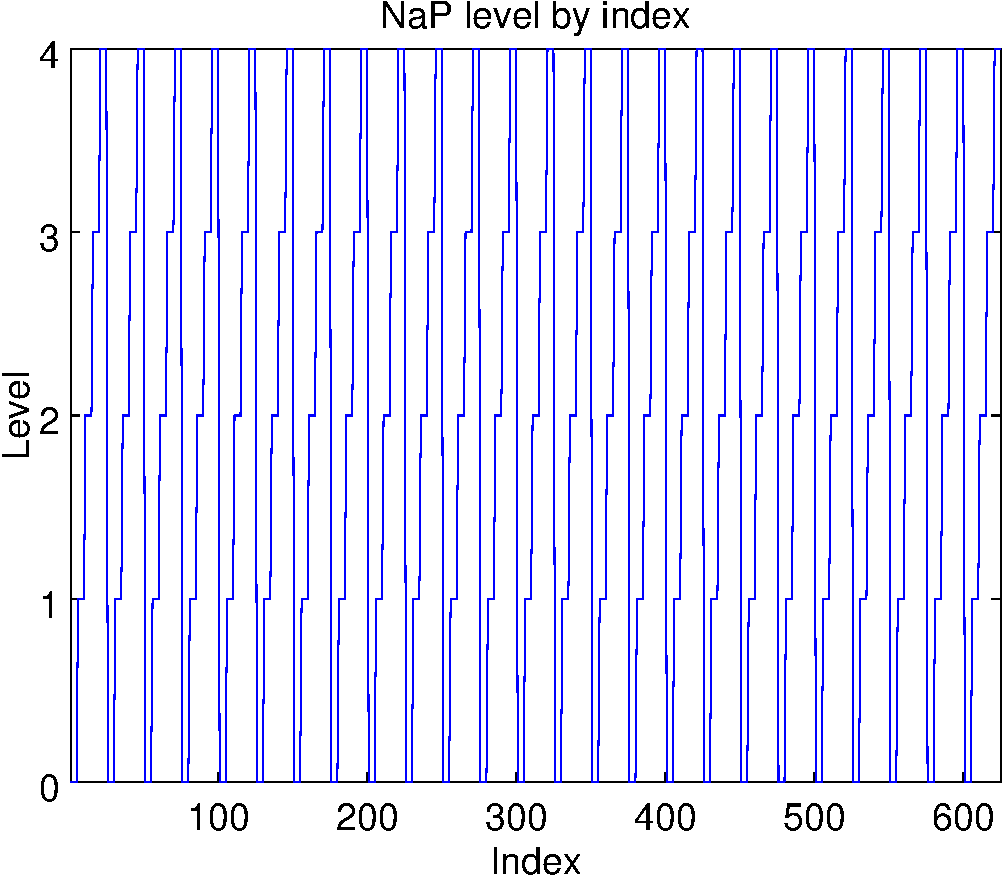
\includegraphics[scale=.32]{NaPfrequency.pdf}
  \end{center}
\end{frame}

\begin{frame}\frametitle{Indexing}
  \begin{center}
    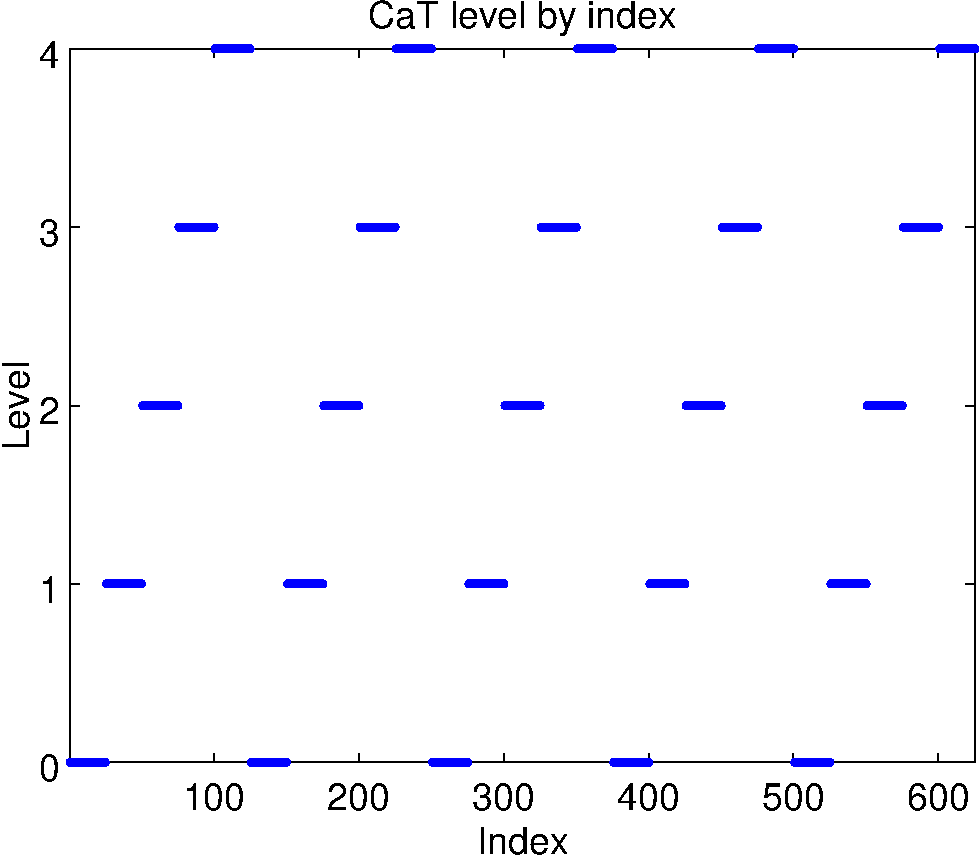
\includegraphics[scale=.32]{CaTfrequency.pdf}%
    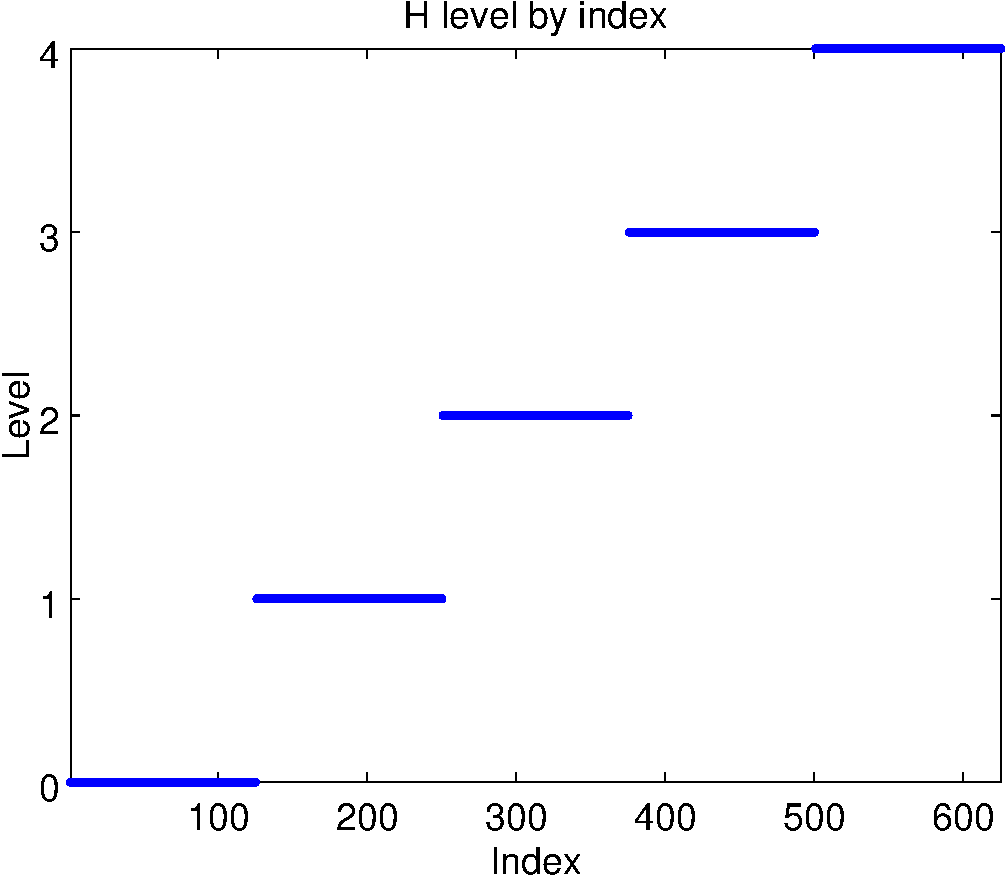
\includegraphics[scale=.32]{Hfrequency.pdf}
  \end{center}
\end{frame}

\section{Results}

\begin{frame}\frametitle{Areas to avoid}
  Bursting fails in the following elements:
  \vspace{1em}

  % $$1 2 3 4 5 126 127 128 129 130 251 252 253 260 376$$


         \begin{tabular}{c c c c c c}

          & 1 & 2 & 3 & 4 & 5 \\

          & 126 & 127 & 128 & 129 & 130 \\

          & 251 & 252 & 253 & 260 & 376  \\
         \end{tabular}

  \vspace{1em}
  These elements are all elements where CaT and NaP are both at their lowest values
\end{frame}

\begin{frame}\frametitle{Burst Duration}
  \begin{center}
    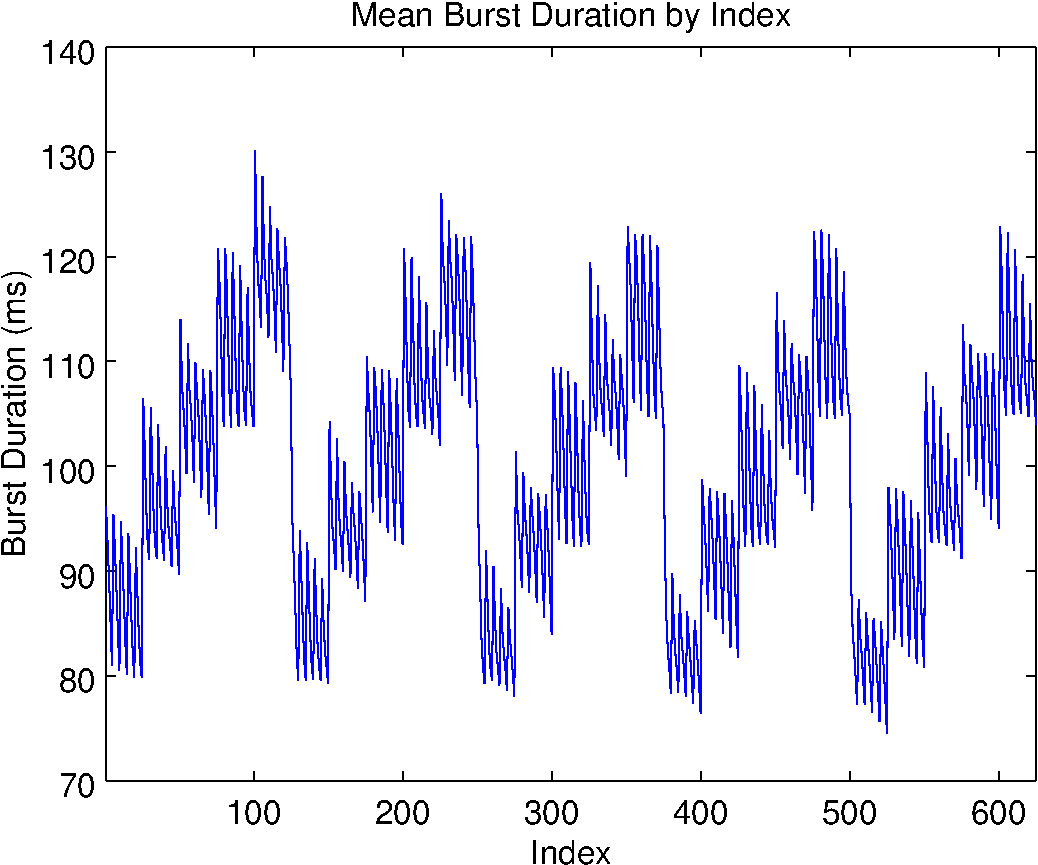
\includegraphics[scale=.32]{BurstDuration.pdf}%
    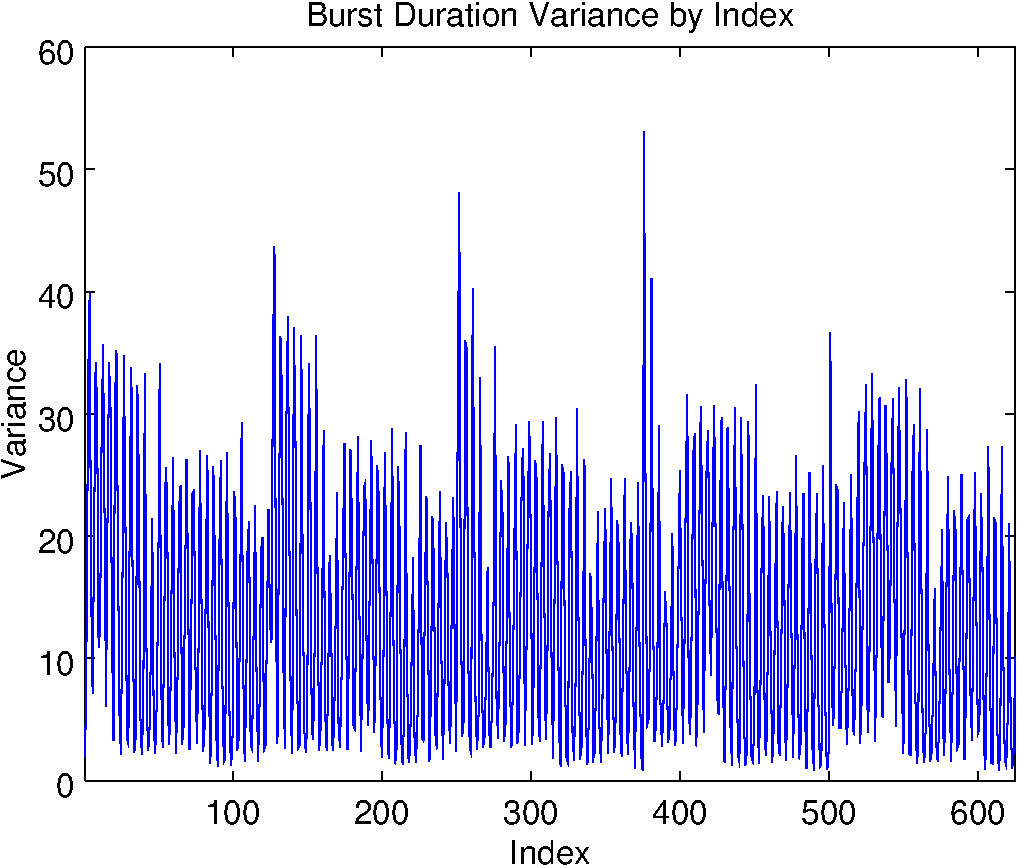
\includegraphics[scale=.32]{BurstDurationVariance.pdf}
  \end{center}
\end{frame}

\begin{frame}\frametitle{Burst Frequency}
  \begin{center}
    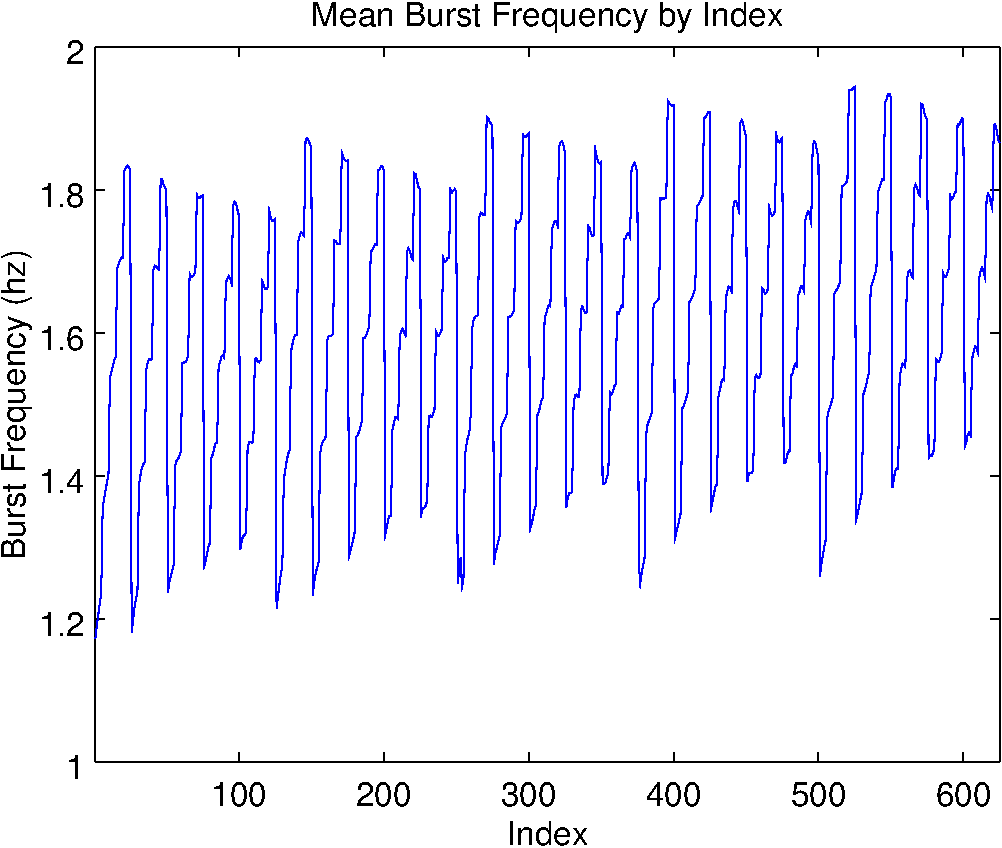
\includegraphics[scale=.32]{BurstFrequency.pdf}%
    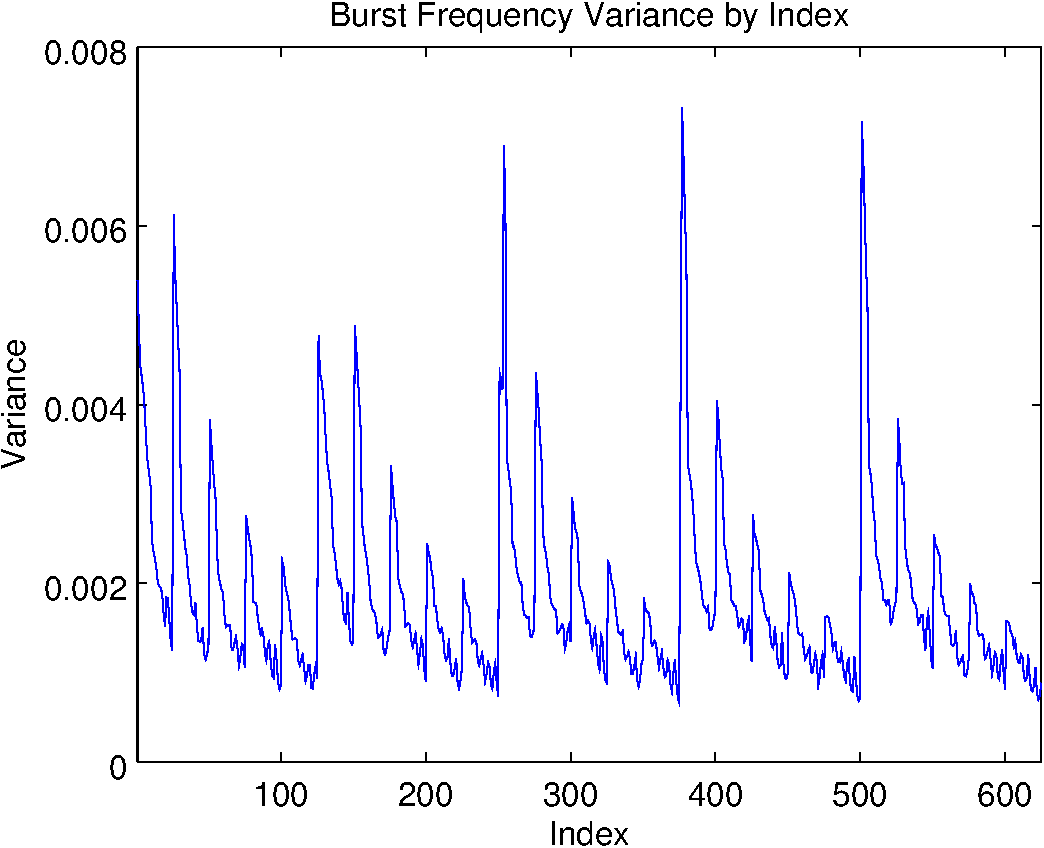
\includegraphics[scale=.32]{BurstFrequencyVariance.pdf}
  \end{center}
\end{frame}

\begin{frame}\frametitle{Spikes Per Burst}
  \begin{center}
    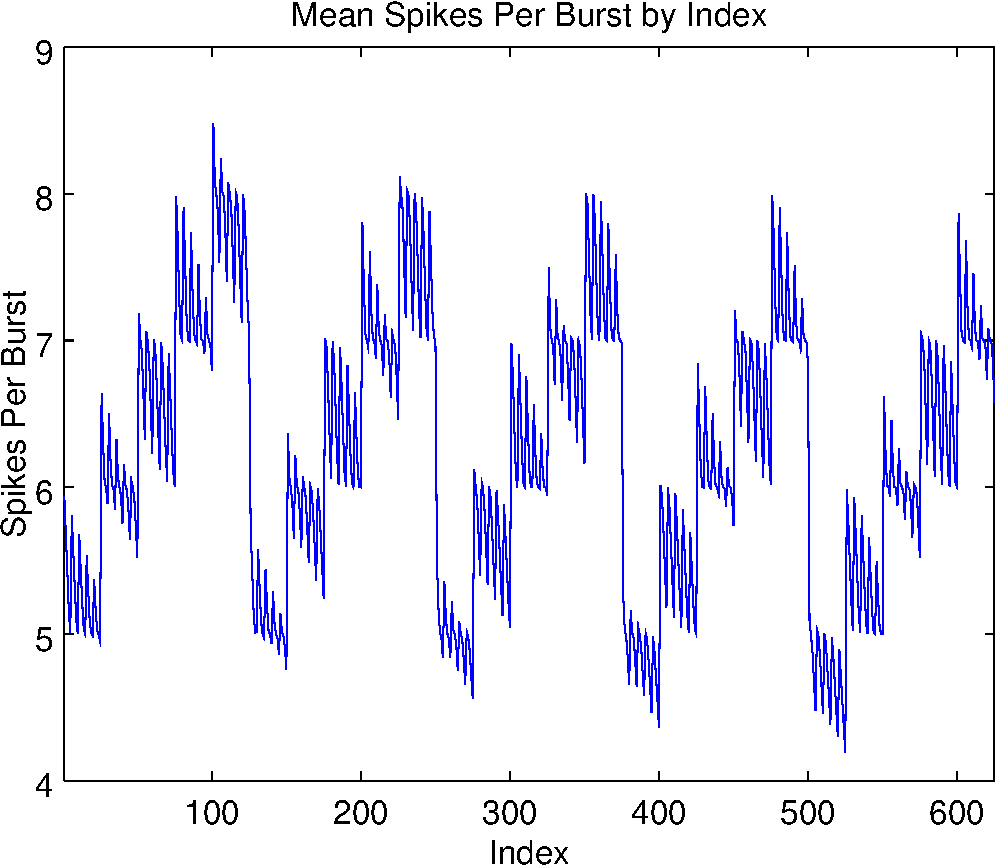
\includegraphics[scale=.32]{SpikesPerBurst.pdf}%
    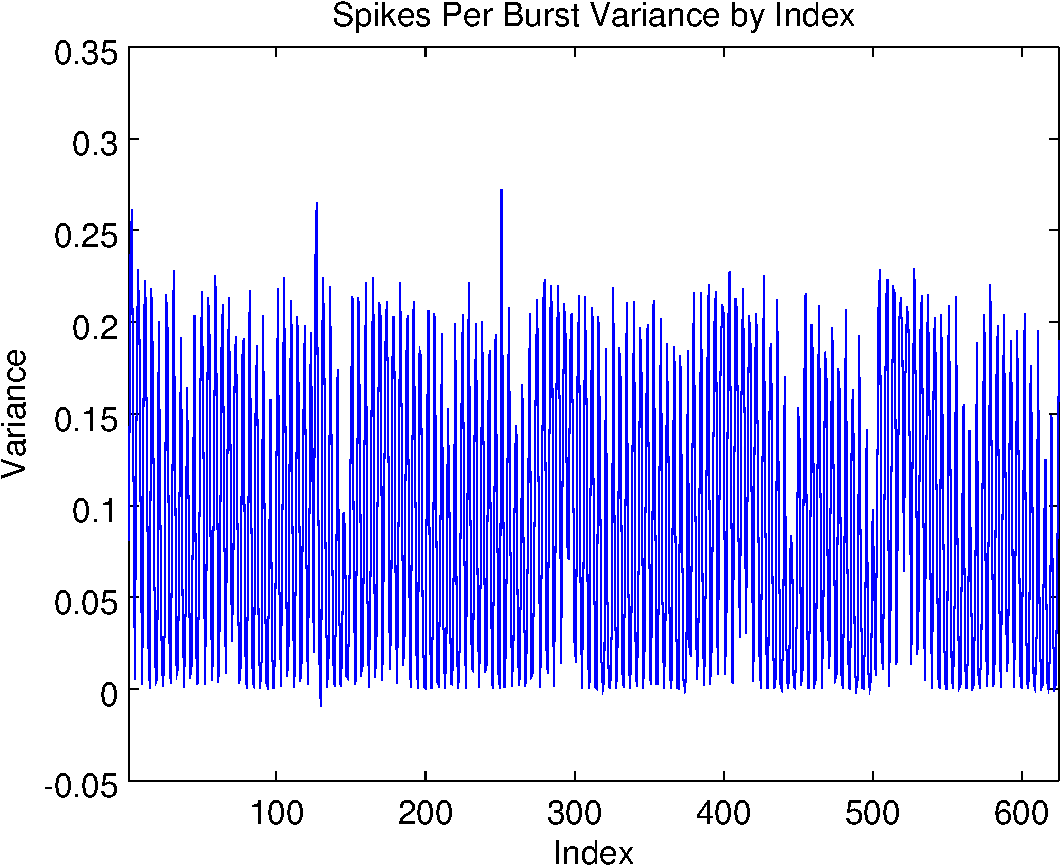
\includegraphics[scale=.32]{SpikesPerBurstVariance.pdf}
  \end{center}
\end{frame}

\begin{frame}\frametitle{Minimum Membrane Potential}
  \begin{center}
    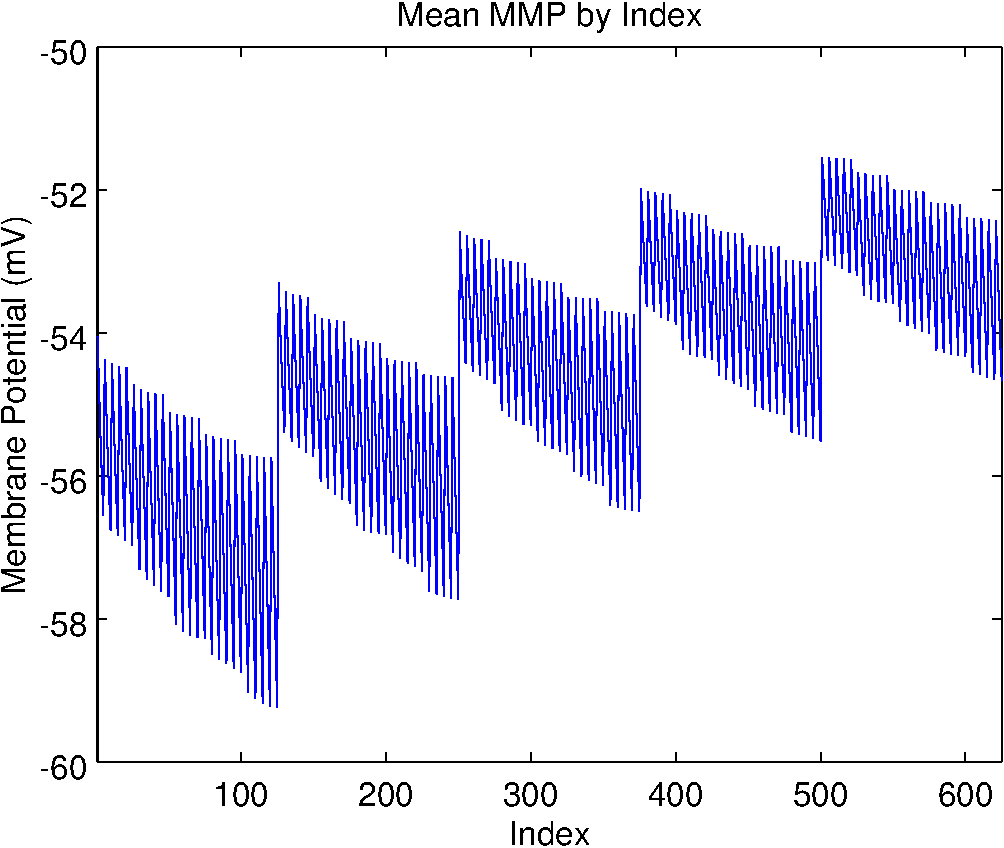
\includegraphics[scale=.32]{MMP.pdf}%
    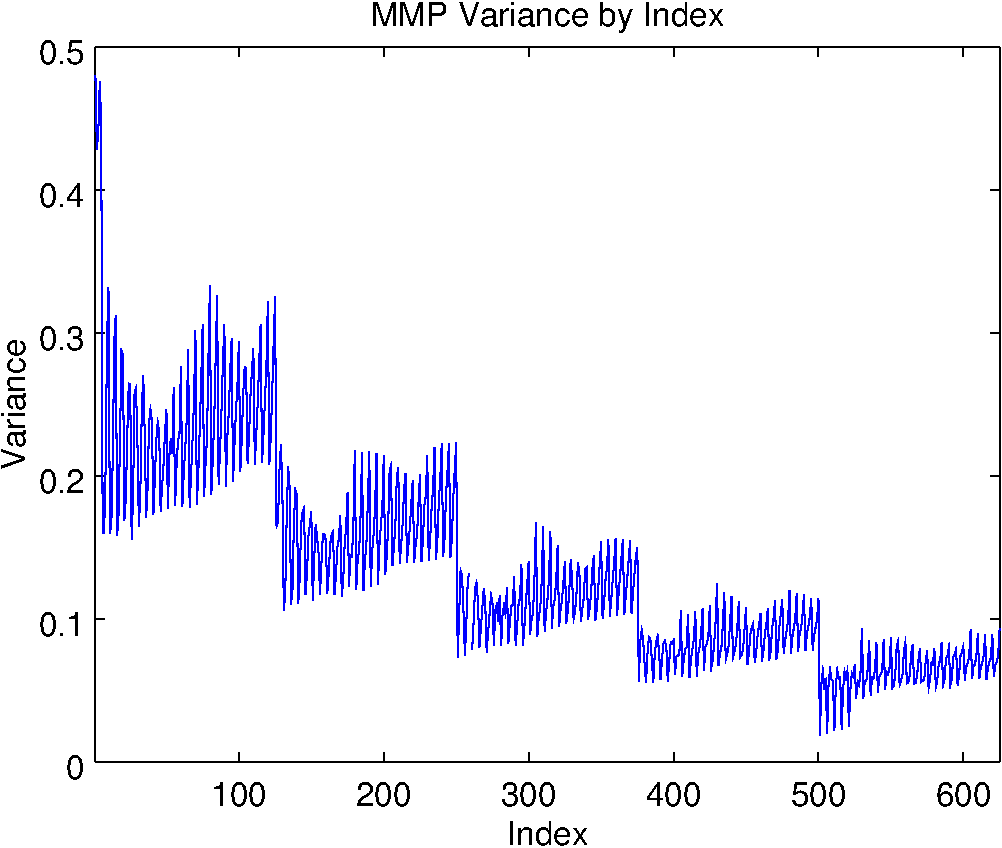
\includegraphics[scale=.32]{MMPVariance.pdf}
  \end{center}
\end{frame}

\begin{frame}\frametitle{Average Membrane Potential}
  \begin{center}
    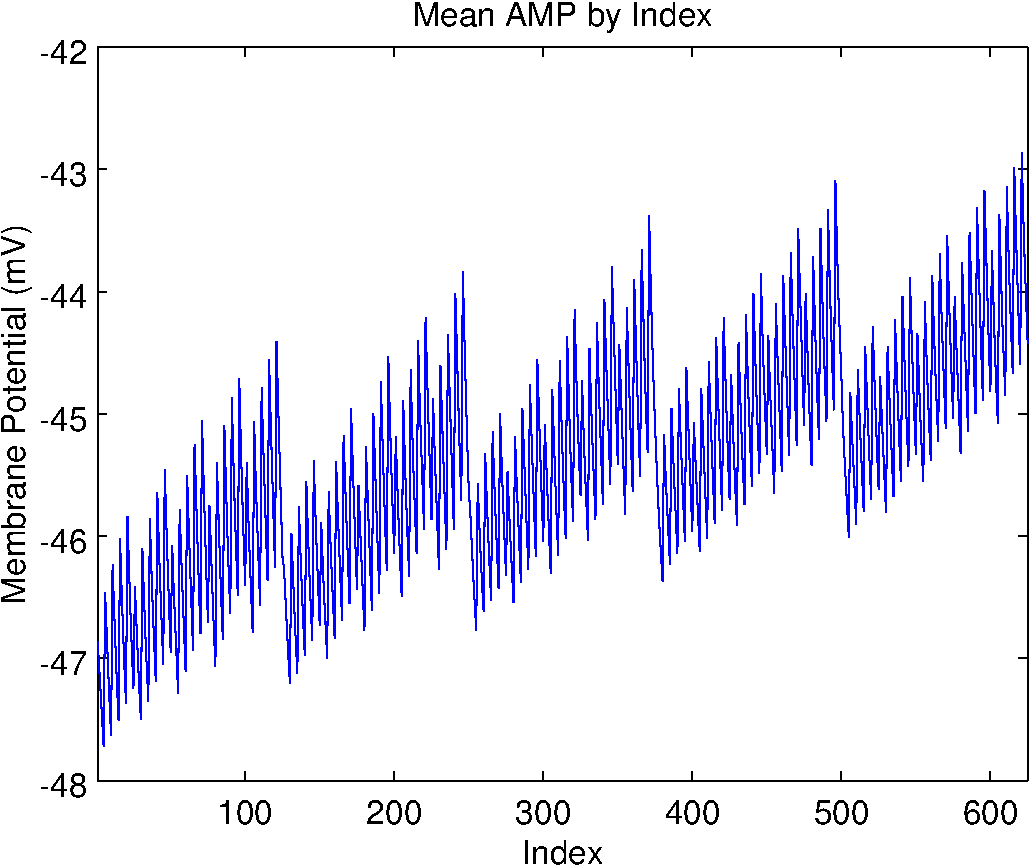
\includegraphics[scale=.32]{AMP.pdf}%
    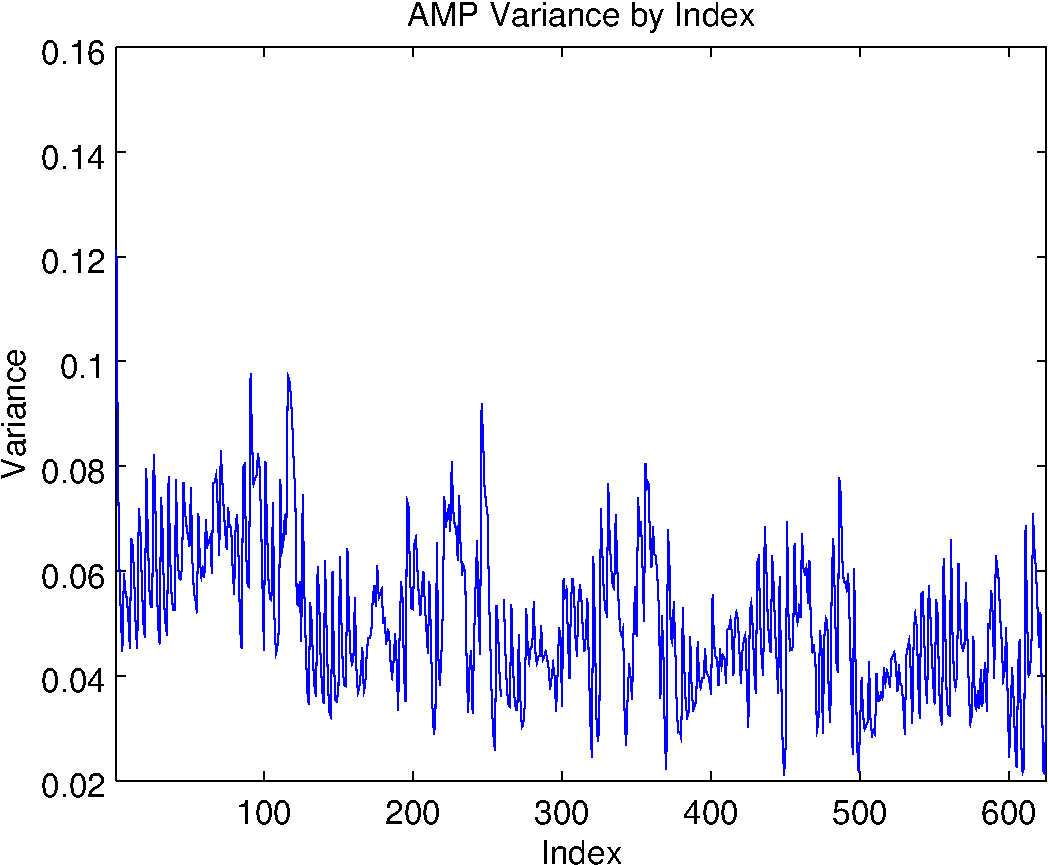
\includegraphics[scale=.32]{AMPVariance.pdf}
  \end{center}
\end{frame}

\begin{frame}\frametitle{Peak Firing Rate}
  \begin{center}
    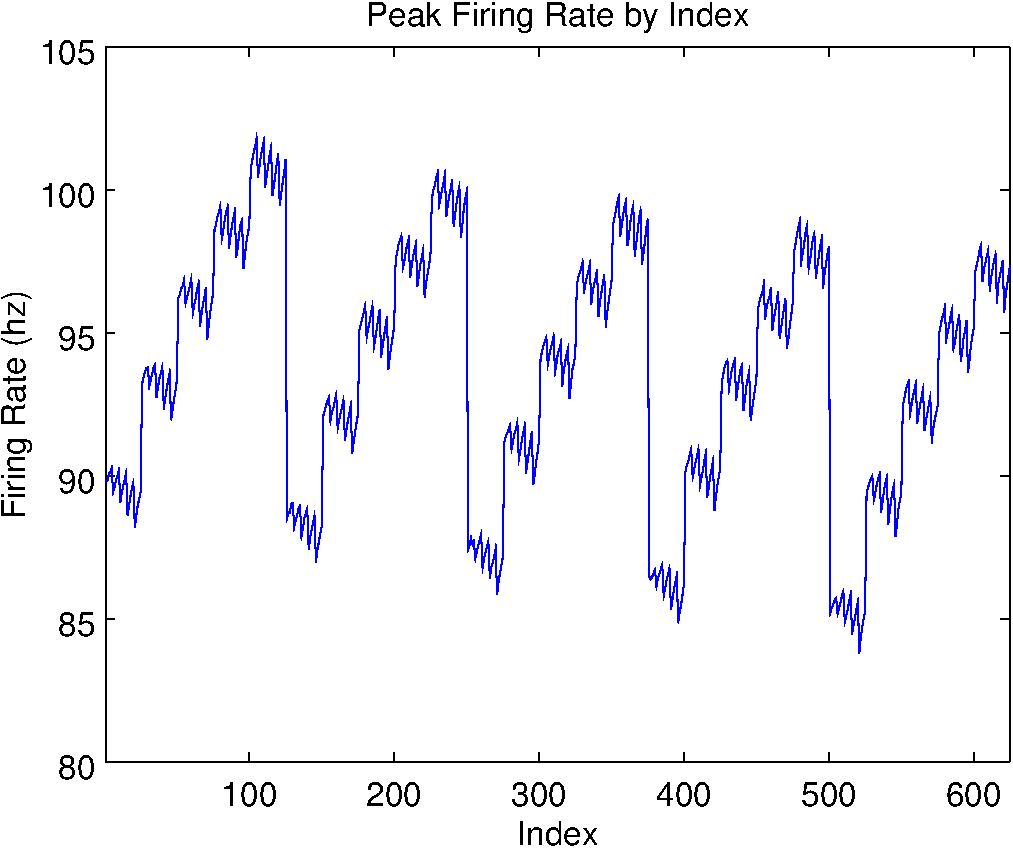
\includegraphics[scale=.32]{PeakFiringRate.pdf}%
    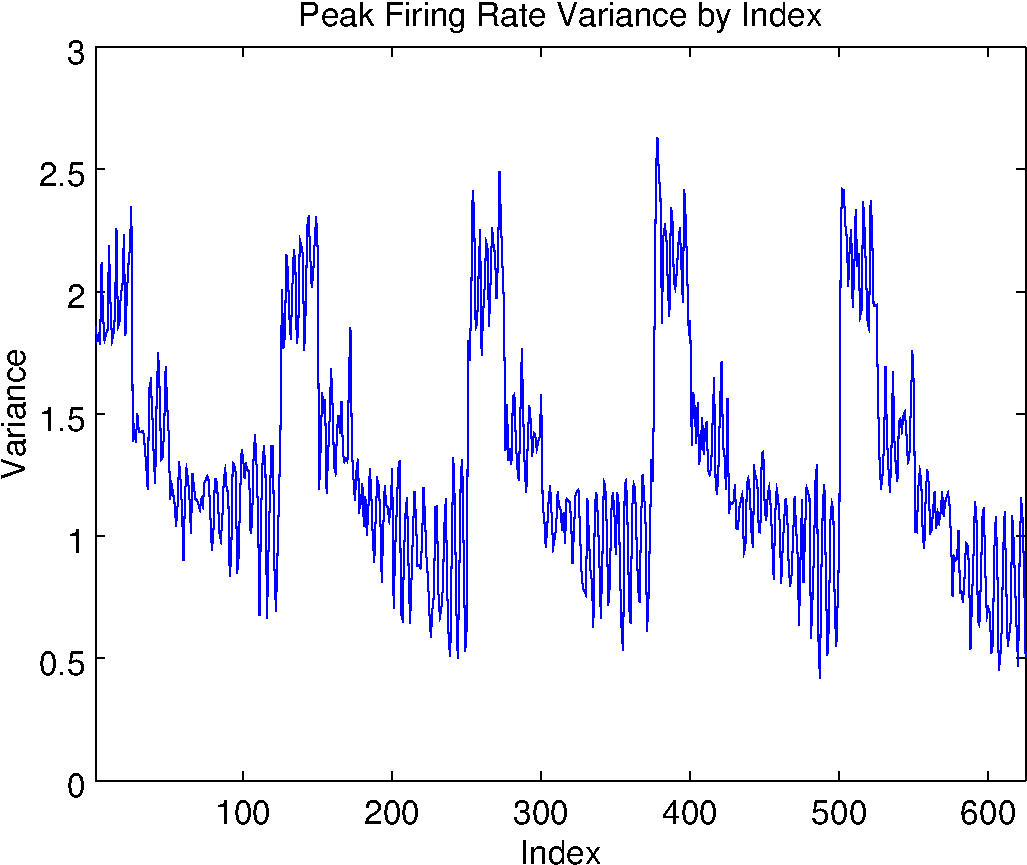
\includegraphics[scale=.32]{PeakFiringRateVariance.pdf}
  \end{center}
\end{frame}

\begin{frame}\frametitle{Average Firing Rate}
  \begin{center}
    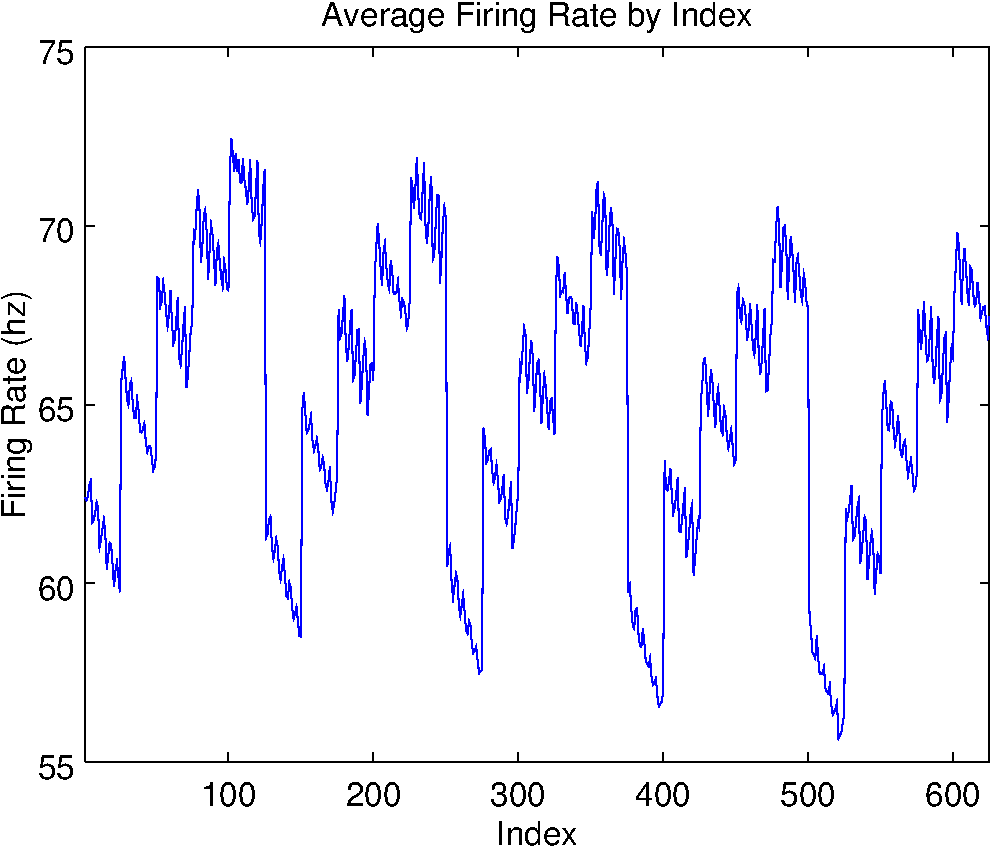
\includegraphics[scale=.32]{AverageFiringRate.pdf}%
    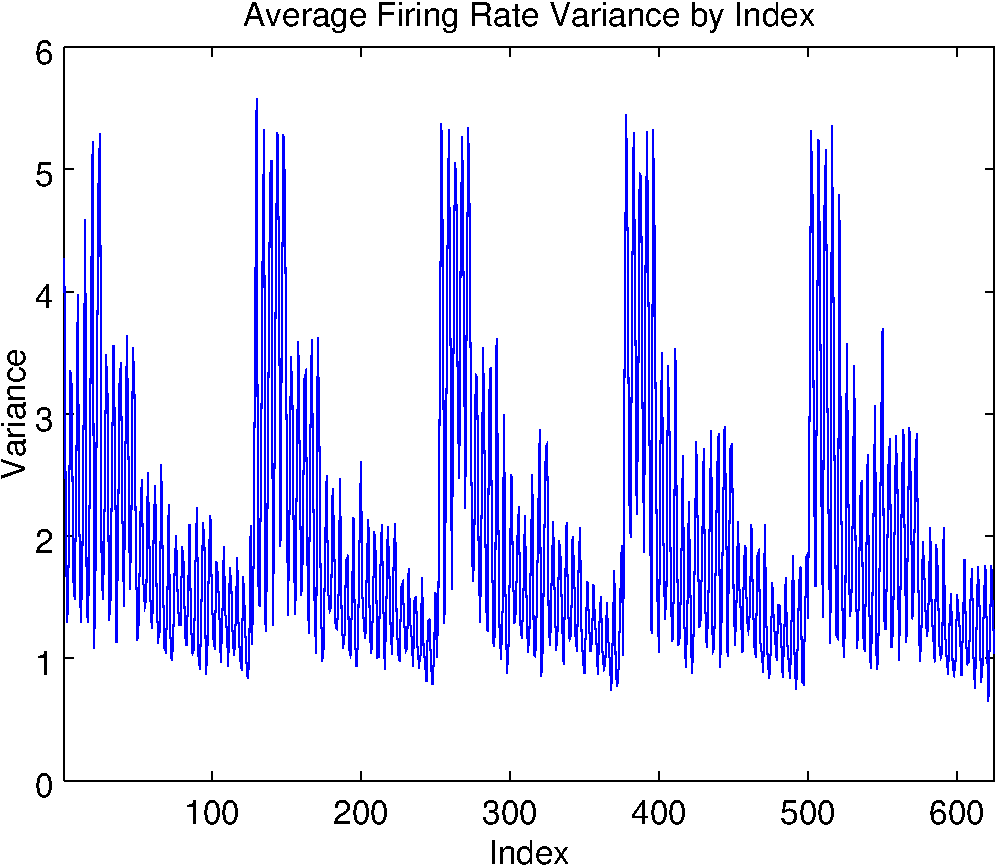
\includegraphics[scale=.32]{AverageFiringRateVariance.pdf}
  \end{center}
\end{frame}

\begin{frame}\frametitle{Least-Squares Projection}
  A least-squares fit of the data onto the space spanned by the 4 basis frequencies gives us a linear estimate of how the output depends on the parameters

  $$A = \left( \begin{array}{c c c c c}
                                       1 & F_1(1) & F_2(1) & F_3(1) & F_4(1)\\
                                       1 & F_1(2) & F_2(2) & F_3(2) & F_4(2)\\
                                       \vdots & \vdots & \vdots & \vdots & \vdots\\
                                       1 & F_1(625) & F_2(625) & F_3(625) & F_4(625)
                                      \end{array} \right)$$

  \vspace{1em}
  Need to solve

  $$A^TAx = A^Tb$$

\end{frame}

\begin{frame}\frametitle{Burst Duration Projection Example}
  Solving $$A^TAx = A^Tb$$ gives

  $$x =    \left( \begin{array}{c}
          96.77815\\
          -1.59413\\
          7.47555\\
          -0.93524\\
          -3.48193
         \end{array} \right)$$

  Thus, $$BD(i) \approx 96.78 - 1.59F_1(i) + 7.48F_2(i) - .94F_3(i) - 3.48F_4(i)$$
\end{frame}

\begin{frame}\frametitle{Burst Duration vs. Projection}
  \begin{center}
    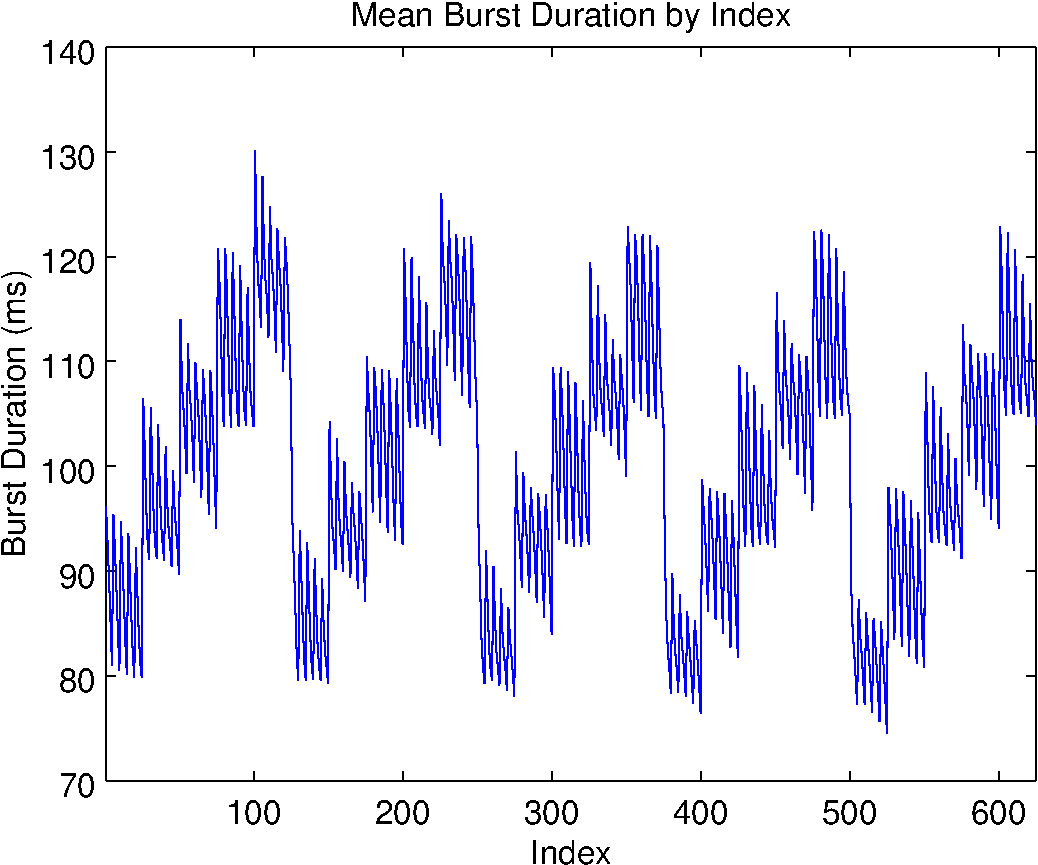
\includegraphics[scale=.32]{BurstDuration.pdf}%
    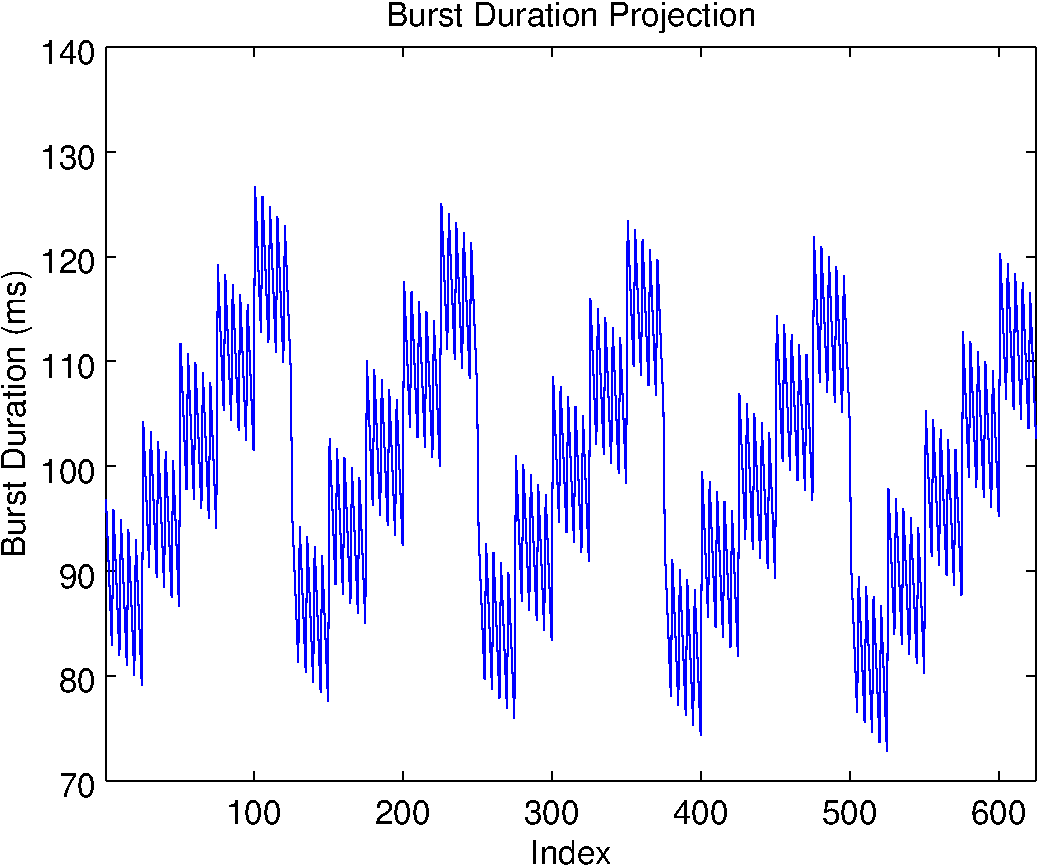
\includegraphics[scale=.32]{BurstDurationProjection.pdf}
  \end{center}
\end{frame}

\begin{frame}\frametitle{Burst Duration Projection Error}
  \begin{center}
    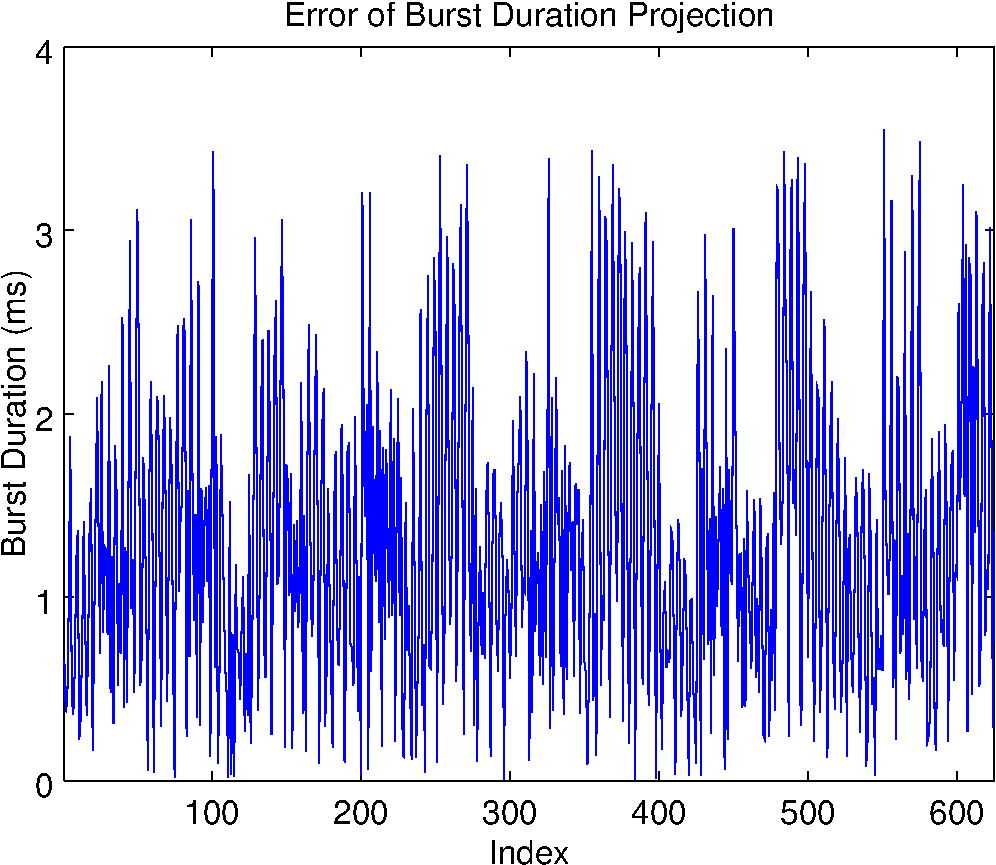
\includegraphics[scale=.5]{BurstDurationError.pdf}%
  \end{center}
\end{frame}

\begin{frame}\frametitle{Burst Frequency vs. Projection}
  \begin{center}
    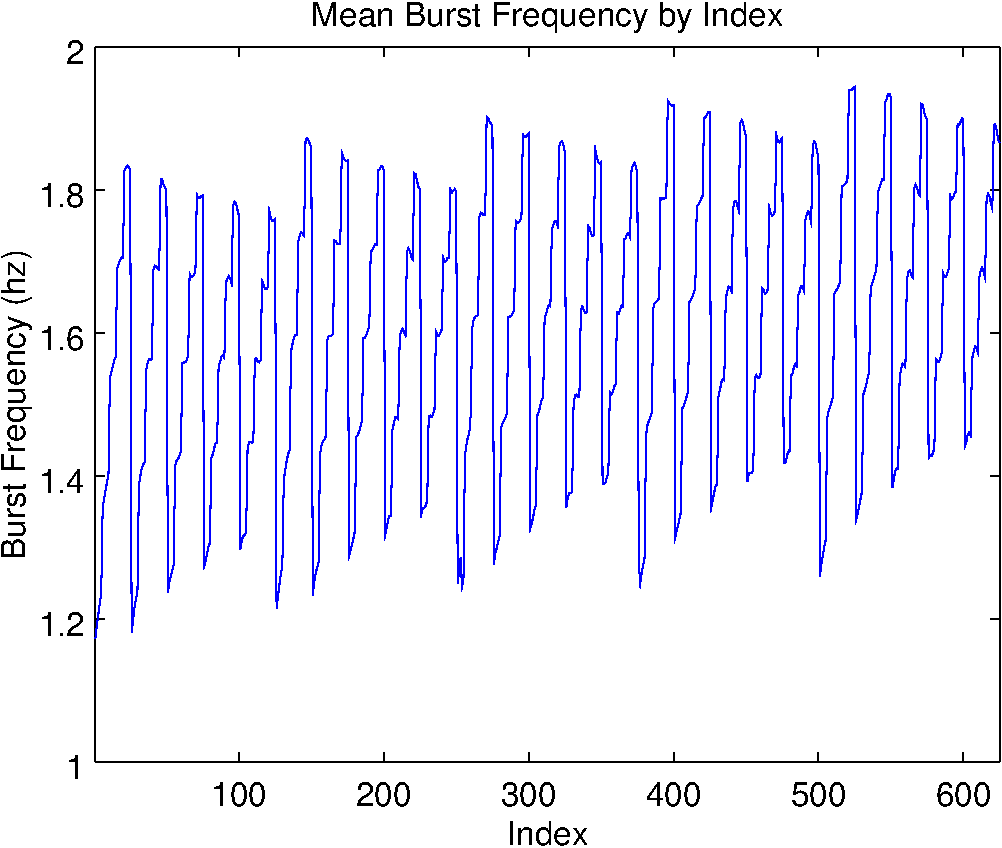
\includegraphics[scale=.32]{BurstFrequency.pdf}%
    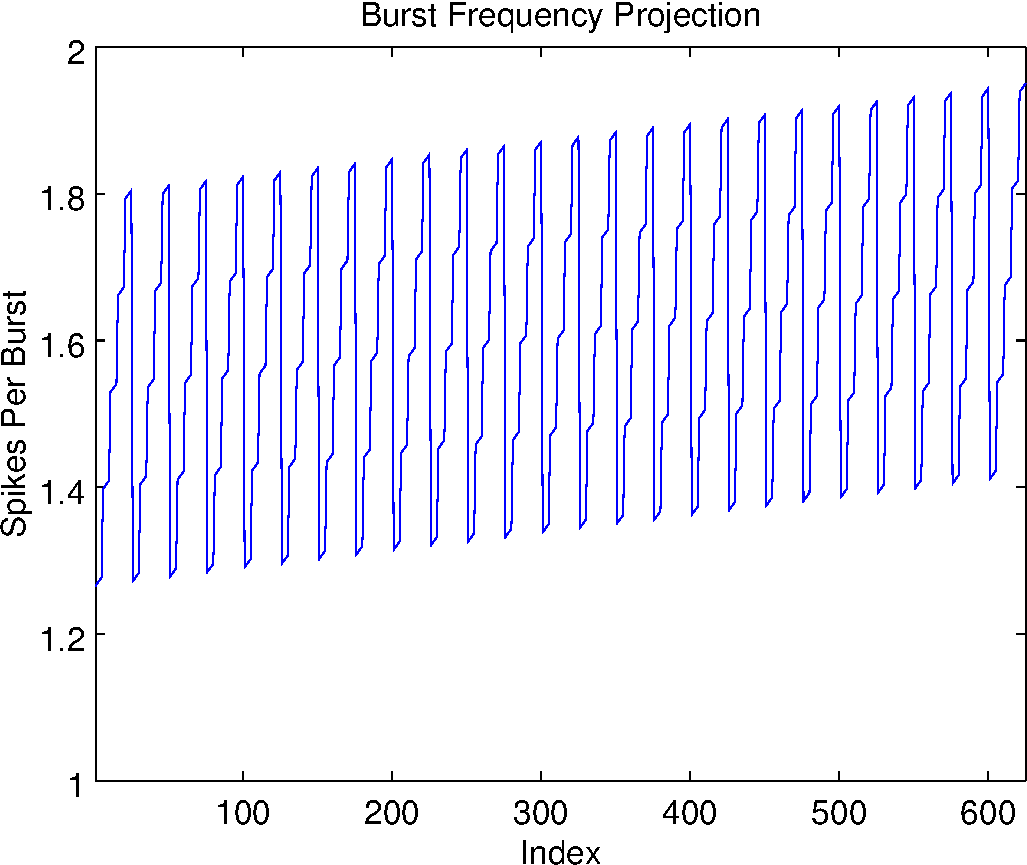
\includegraphics[scale=.32]{BurstFrequencyProjection.pdf}
  \end{center}
\end{frame}

% \begin{frame}\frametitle{Burst Frequency Projection Error}
%   \begin{center}
%     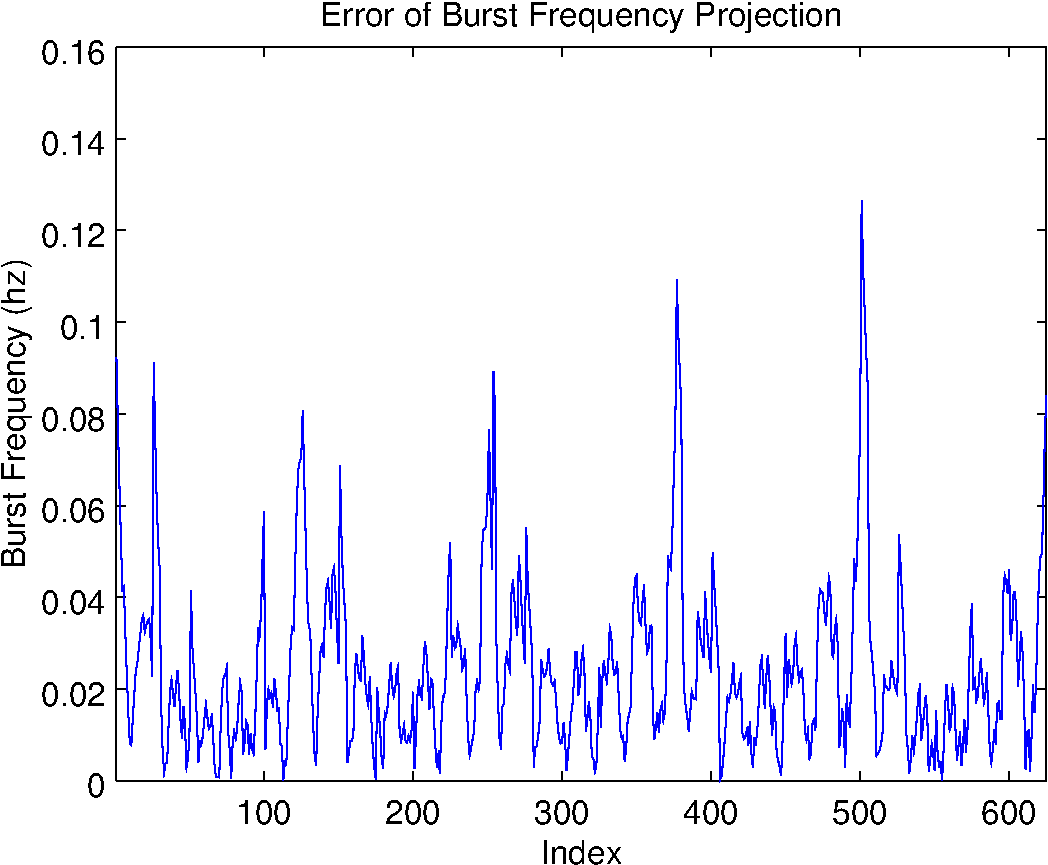
\includegraphics[scale=.5]{BurstFrequencyError.pdf}%
%   \end{center}
% \end{frame}

\begin{frame}\frametitle{Spikes Per Burst vs. Projection}
  \begin{center}
    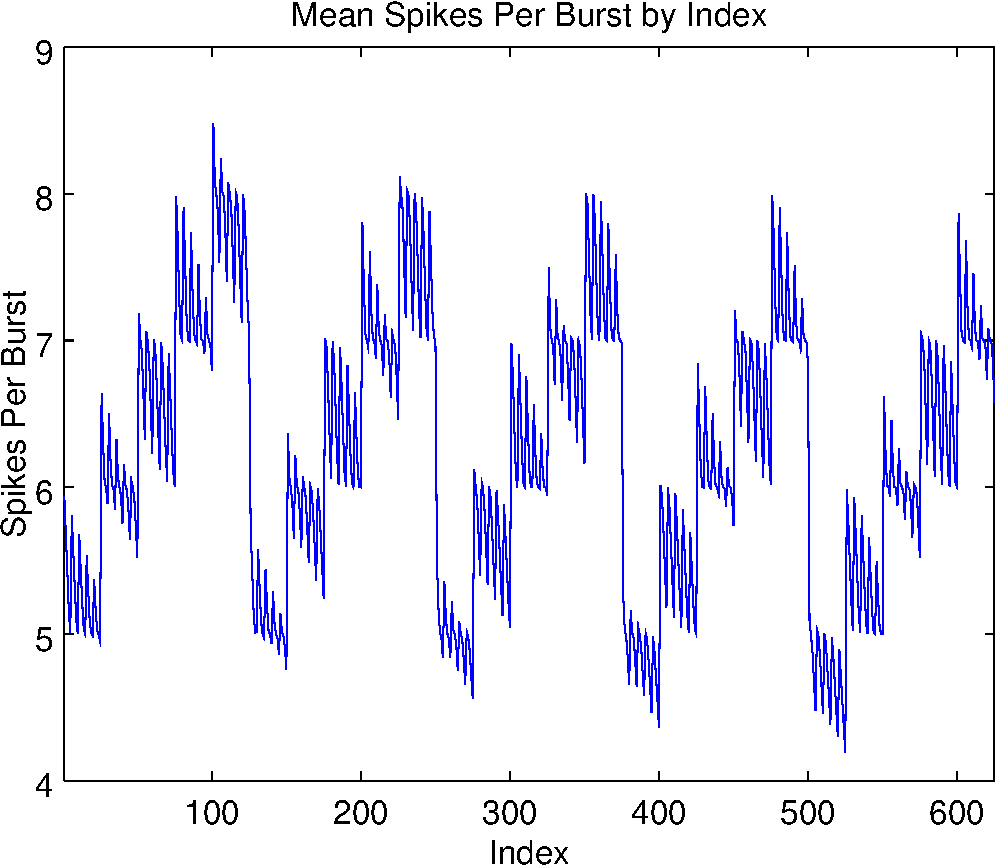
\includegraphics[scale=.32]{SpikesPerBurst.pdf}%
    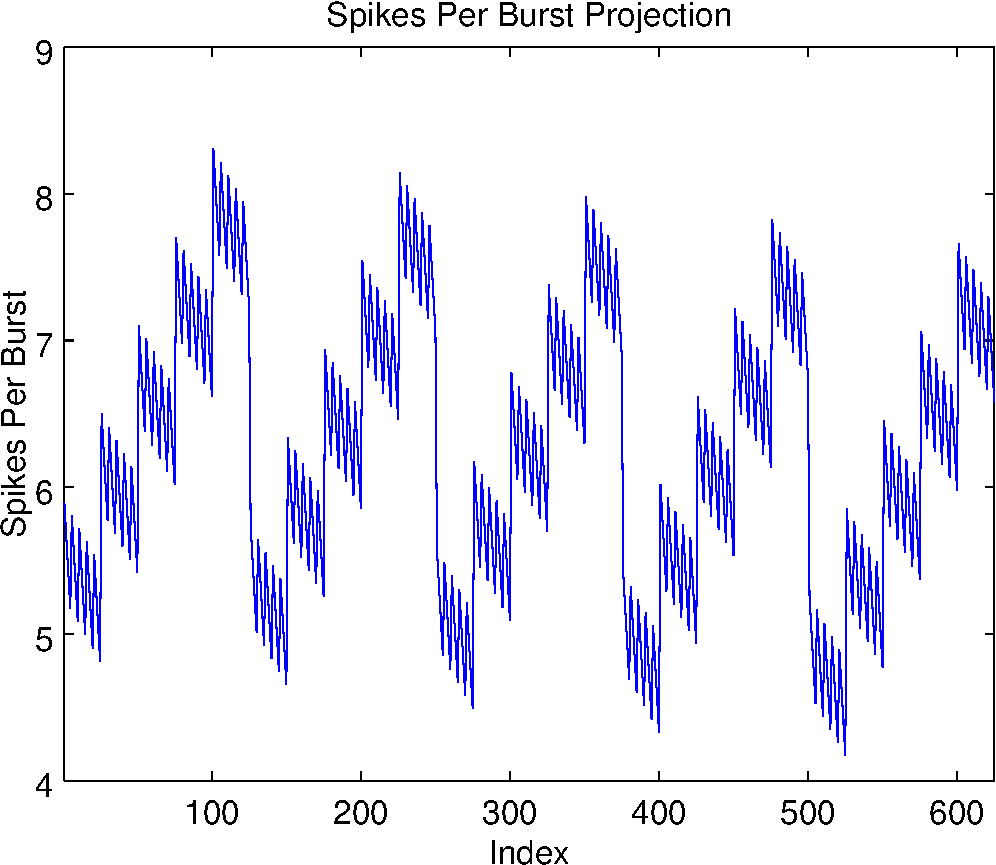
\includegraphics[scale=.32]{SpikesPerBurstProjection.pdf}
  \end{center}
\end{frame}

% \begin{frame}\frametitle{Spikes Per Burst Projection Error}
%   \begin{center}
%     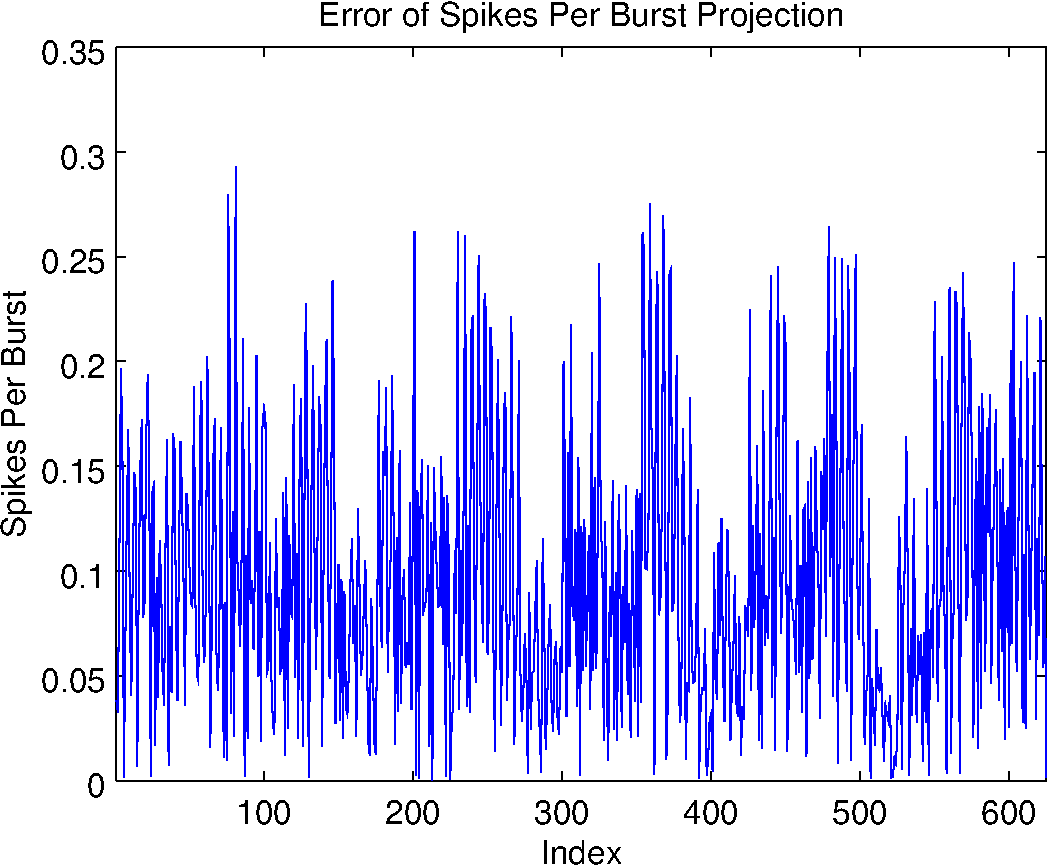
\includegraphics[scale=.5]{SpikesPerBurstError.pdf}%
%   \end{center}
% \end{frame}

\begin{frame}\frametitle{MMP vs. Projection}
  \begin{center}
    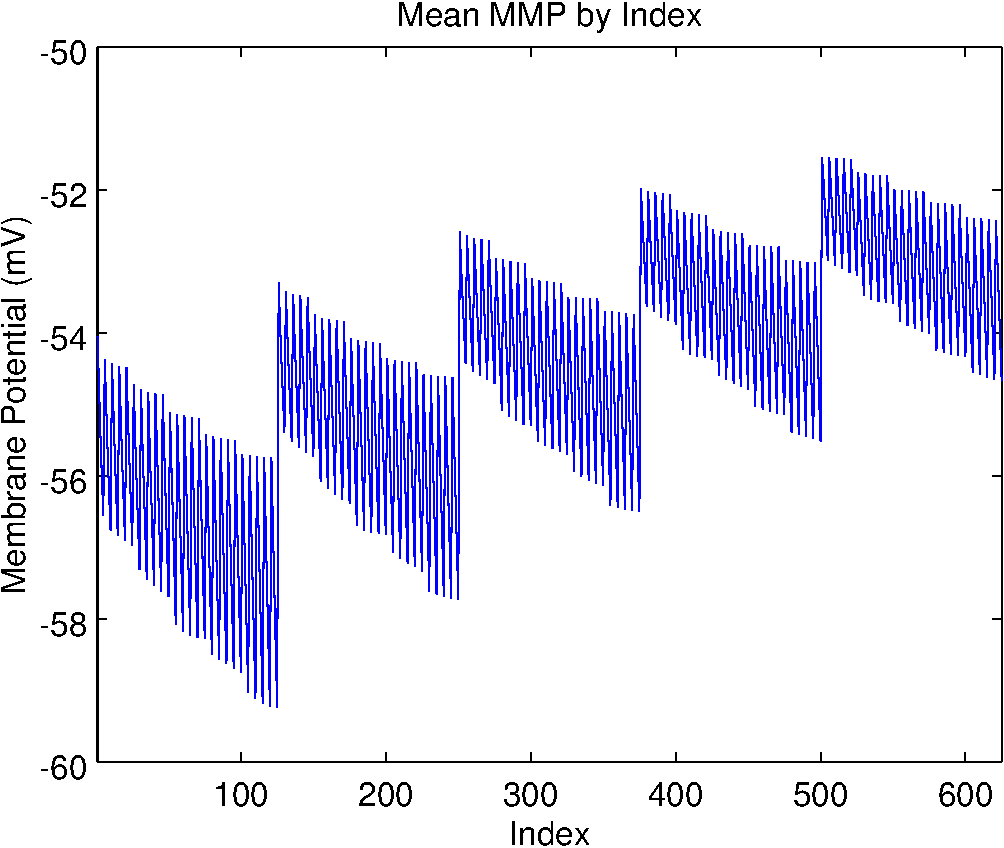
\includegraphics[scale=.32]{MMP.pdf}%
    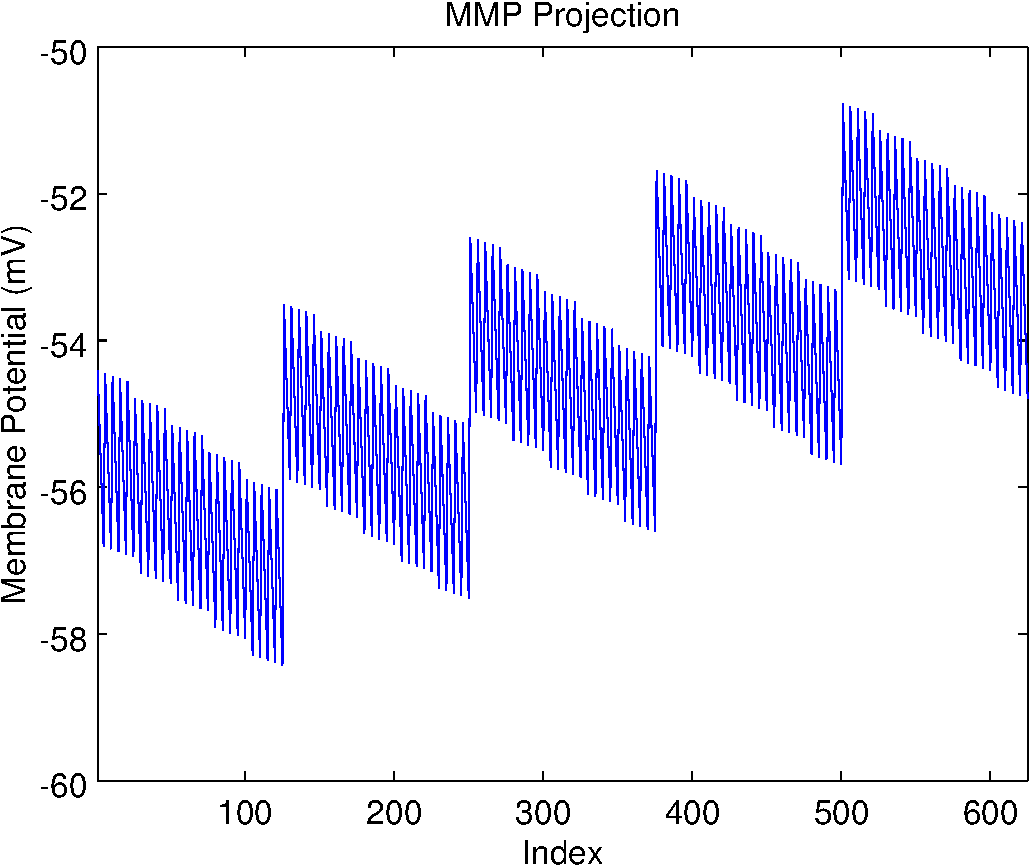
\includegraphics[scale=.32]{MMPProjection.pdf}
  \end{center}
\end{frame}

% \begin{frame}\frametitle{MMP Projection Error}
%   \begin{center}
%     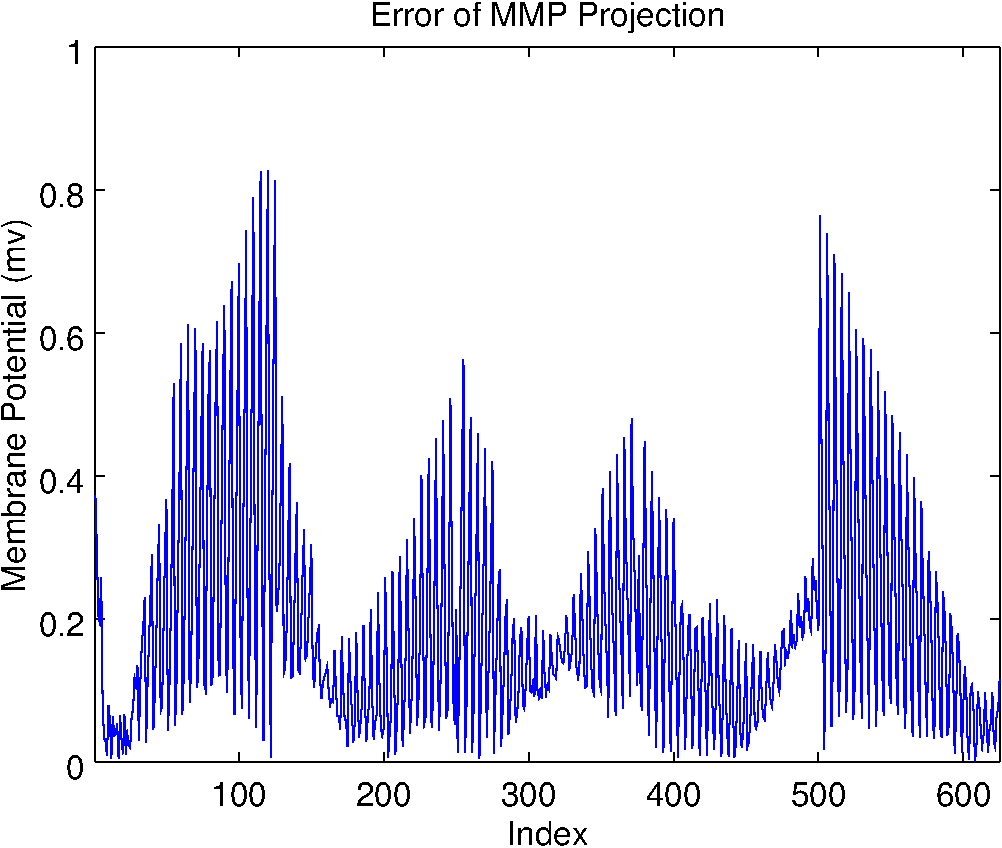
\includegraphics[scale=.5]{MMPError.pdf}%
%   \end{center}
% \end{frame}

\begin{frame}\frametitle{AMP vs. Projection}
  \begin{center}
    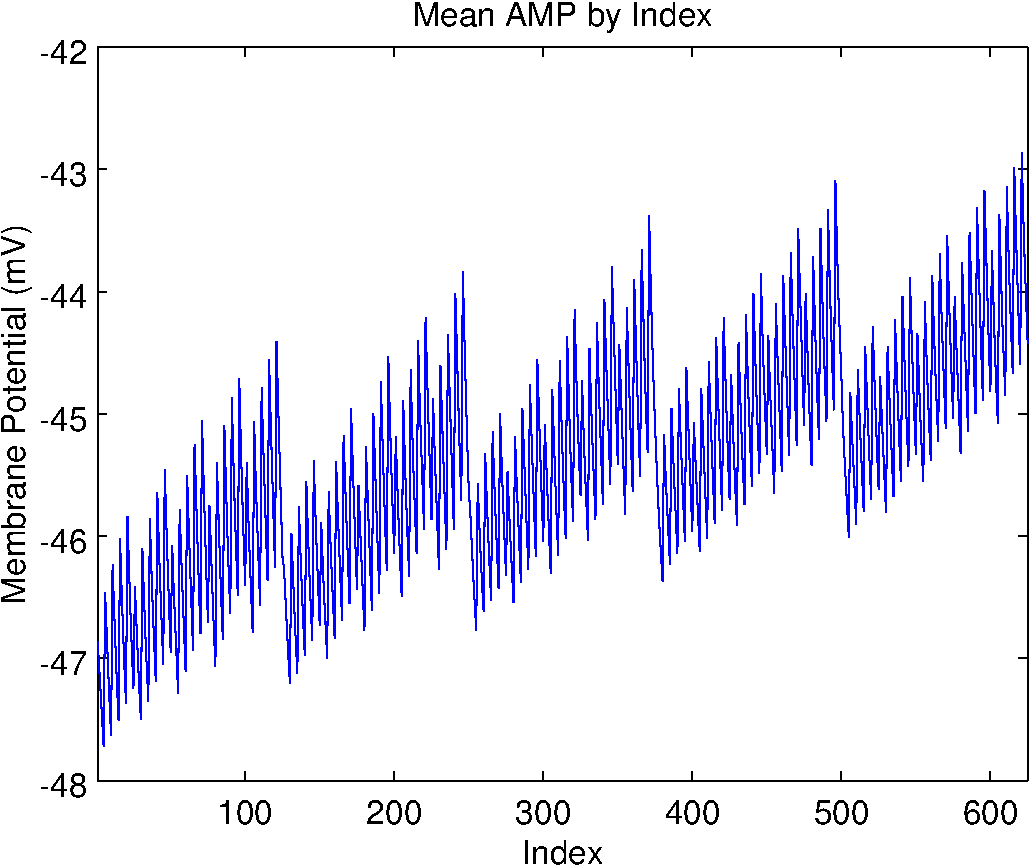
\includegraphics[scale=.32]{AMP.pdf}%
    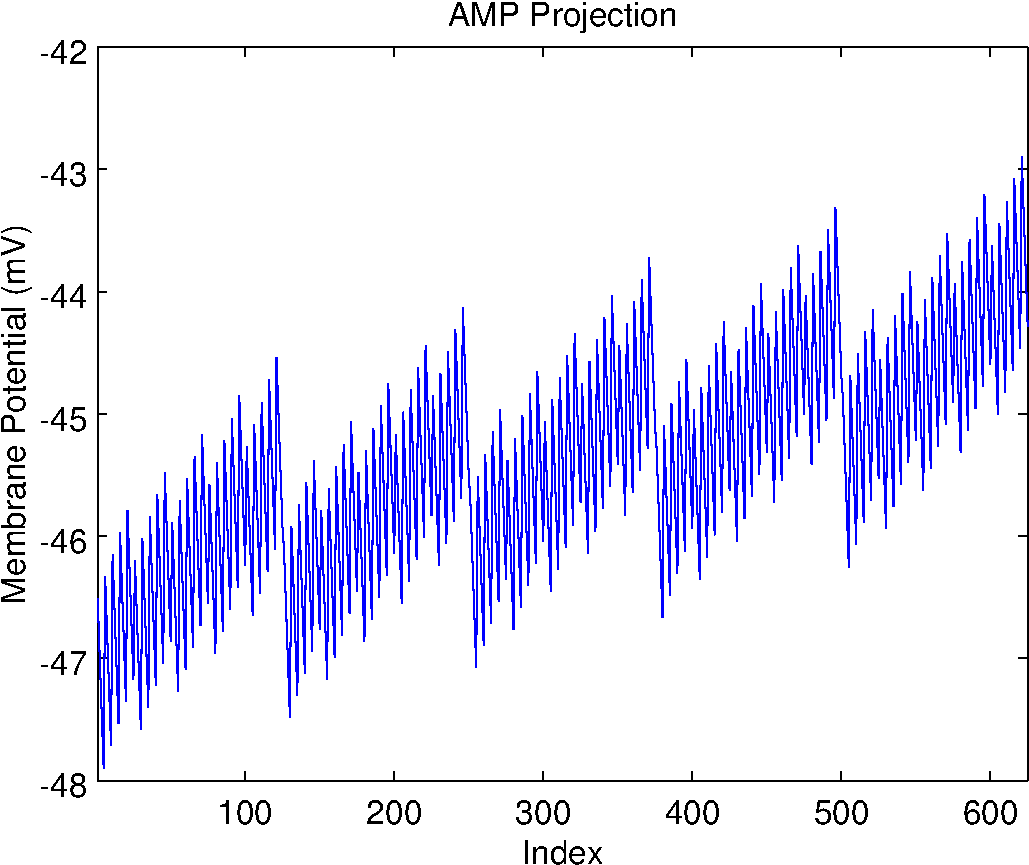
\includegraphics[scale=.32]{AMPProjection.pdf}
  \end{center}
\end{frame}

% \begin{frame}\frametitle{AMP Projection Error}
%   \begin{center}
%     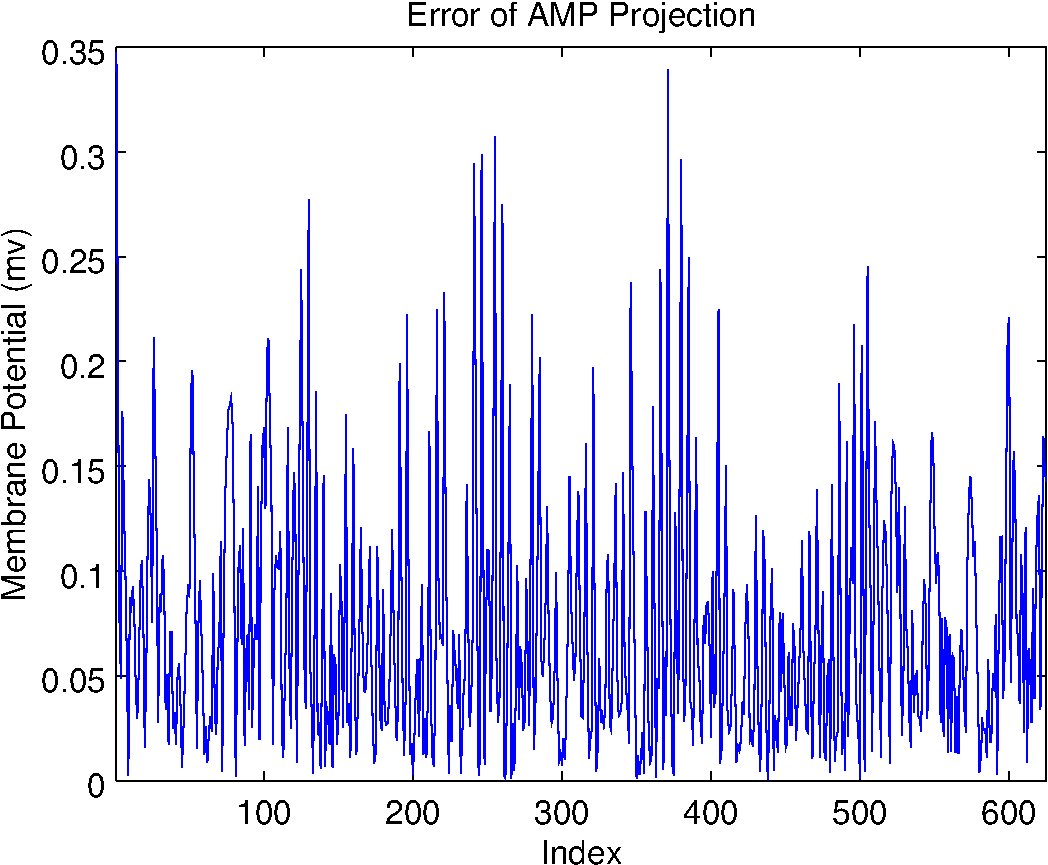
\includegraphics[scale=.5]{AMPError.pdf}%
%   \end{center}
% \end{frame}

\begin{frame}\frametitle{Peak Firing Rate vs. Projection}
  \begin{center}
    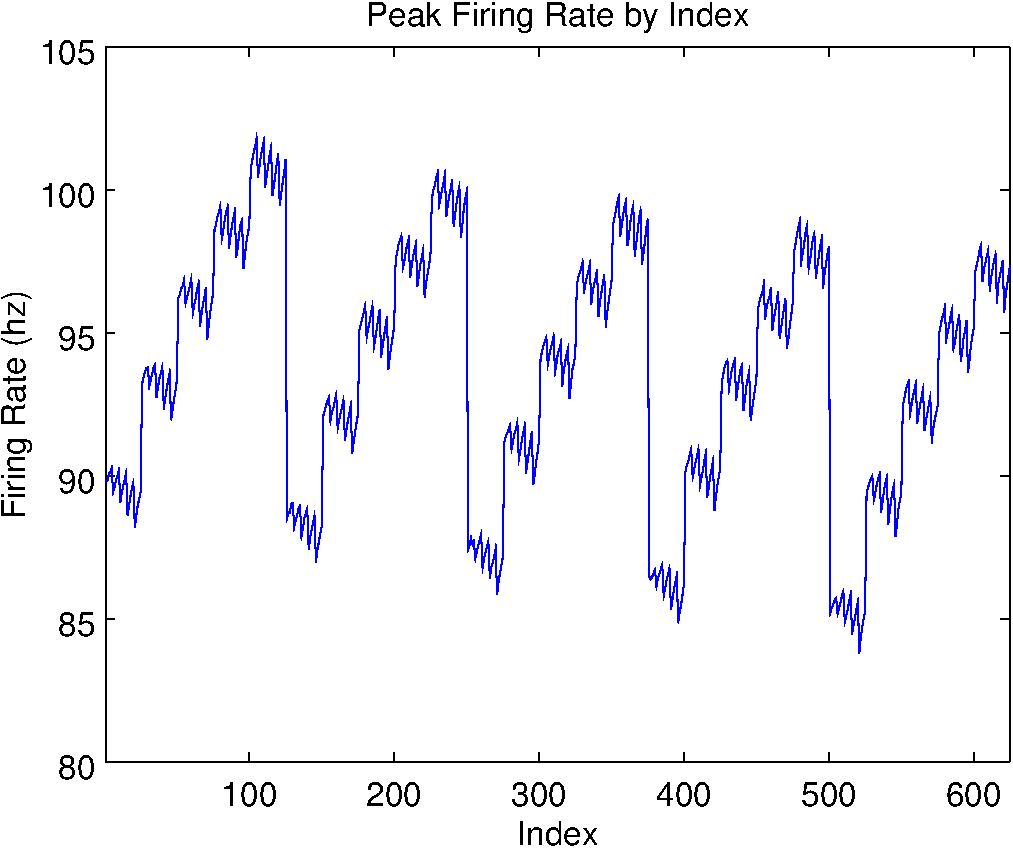
\includegraphics[scale=.32]{PeakFiringRate.pdf}%
    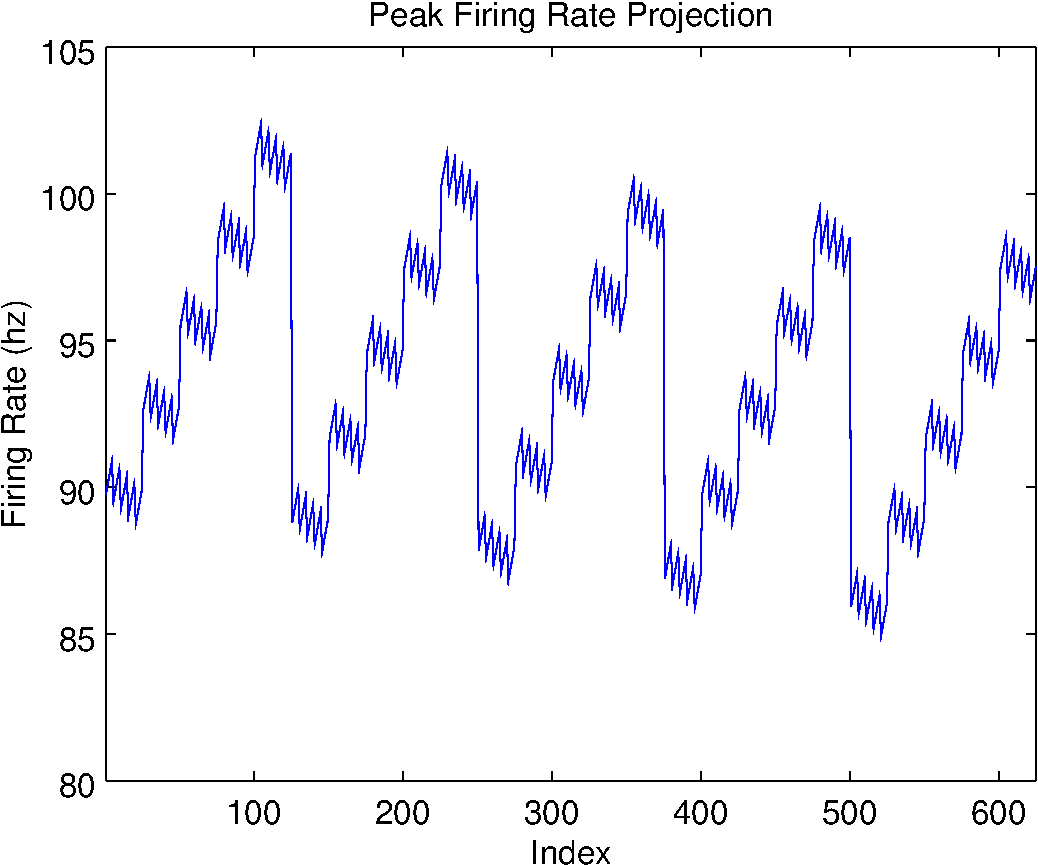
\includegraphics[scale=.32]{PeakFiringRateProjection.pdf}
  \end{center}
\end{frame}

% \begin{frame}\frametitle{Peak Firing Rate Projection Error}
%   \begin{center}
%     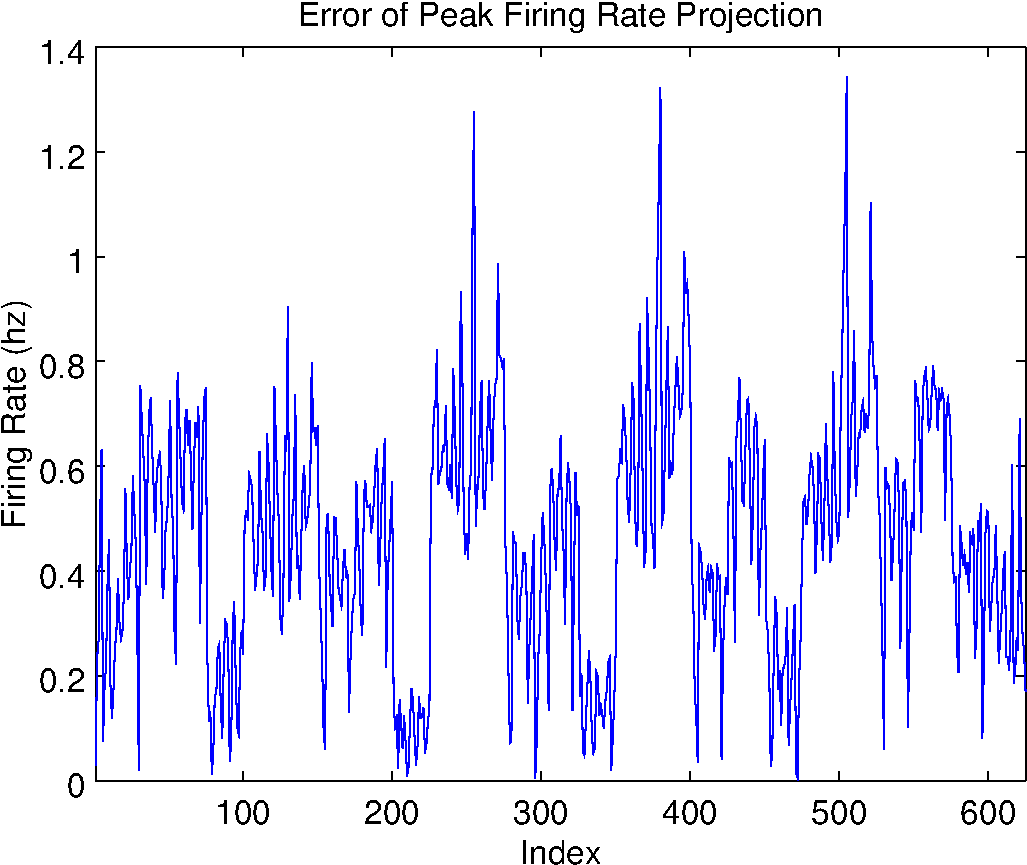
\includegraphics[scale=.5]{PeakFiringRateError.pdf}%
%   \end{center}
% \end{frame}

\begin{frame}\frametitle{Average Firing Rate vs. Projection}
  \begin{center}
    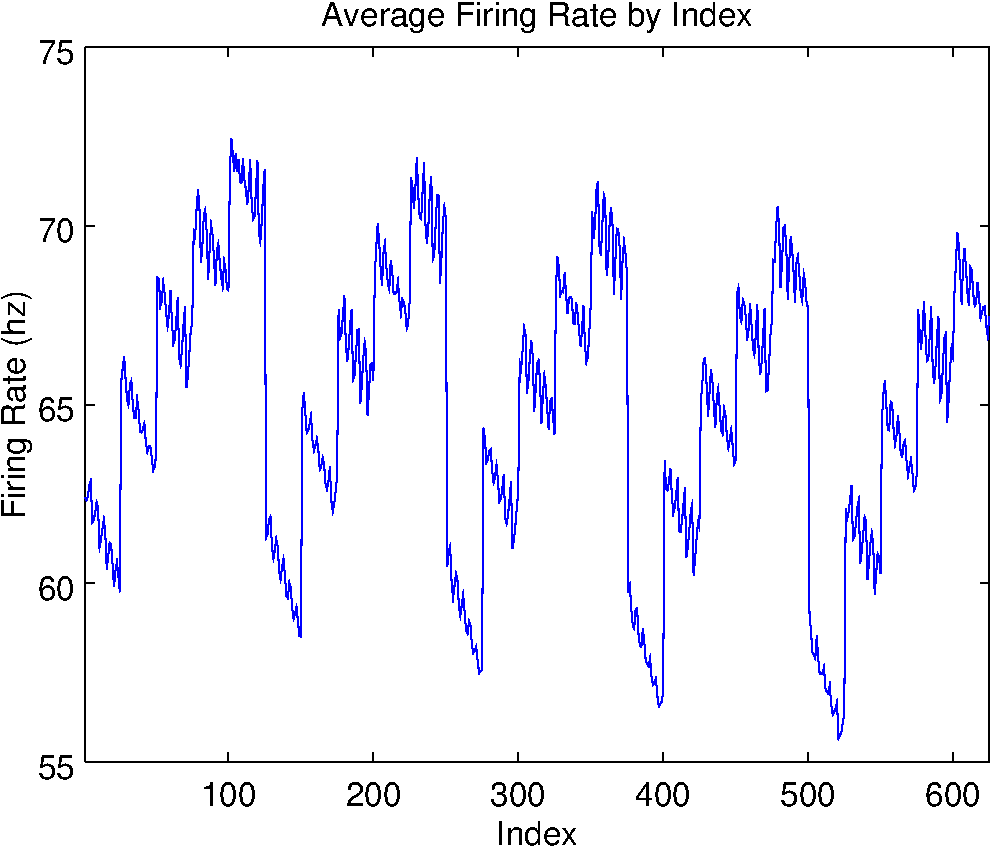
\includegraphics[scale=.32]{AverageFiringRate.pdf}%
    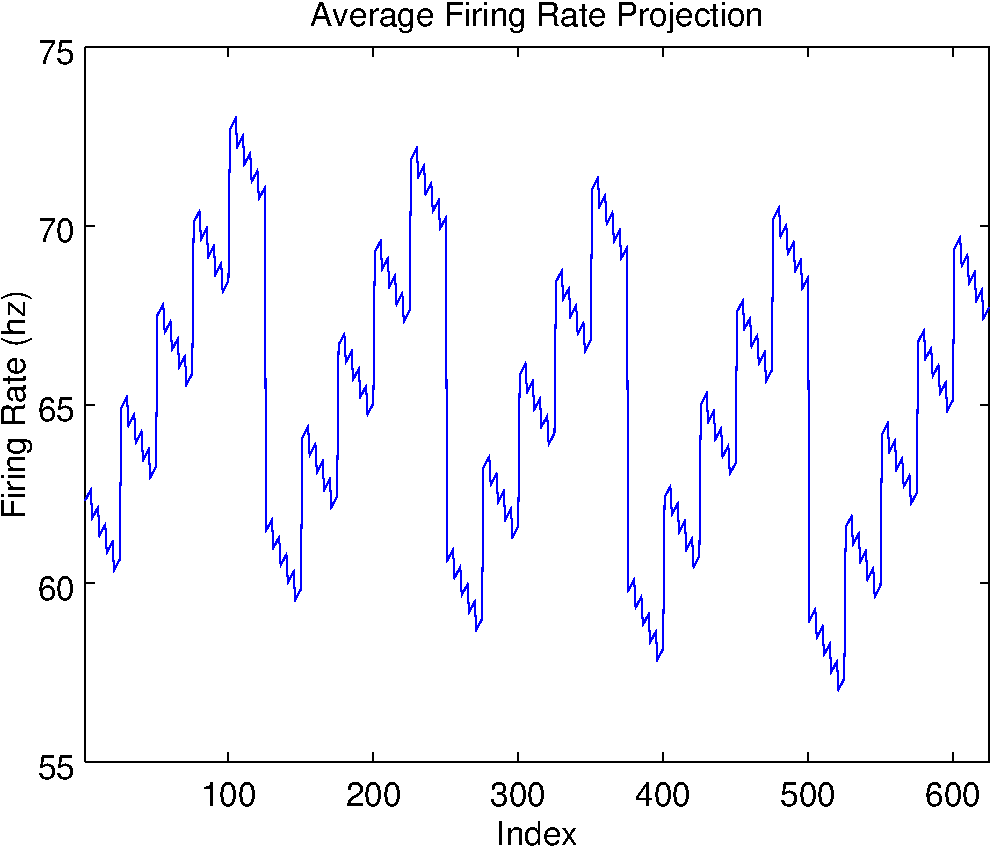
\includegraphics[scale=.32]{AverageFiringRateProjection.pdf}
  \end{center}
\end{frame}

% \begin{frame}\frametitle{Average Firing Rate Projection Error}
%   \begin{center}
%     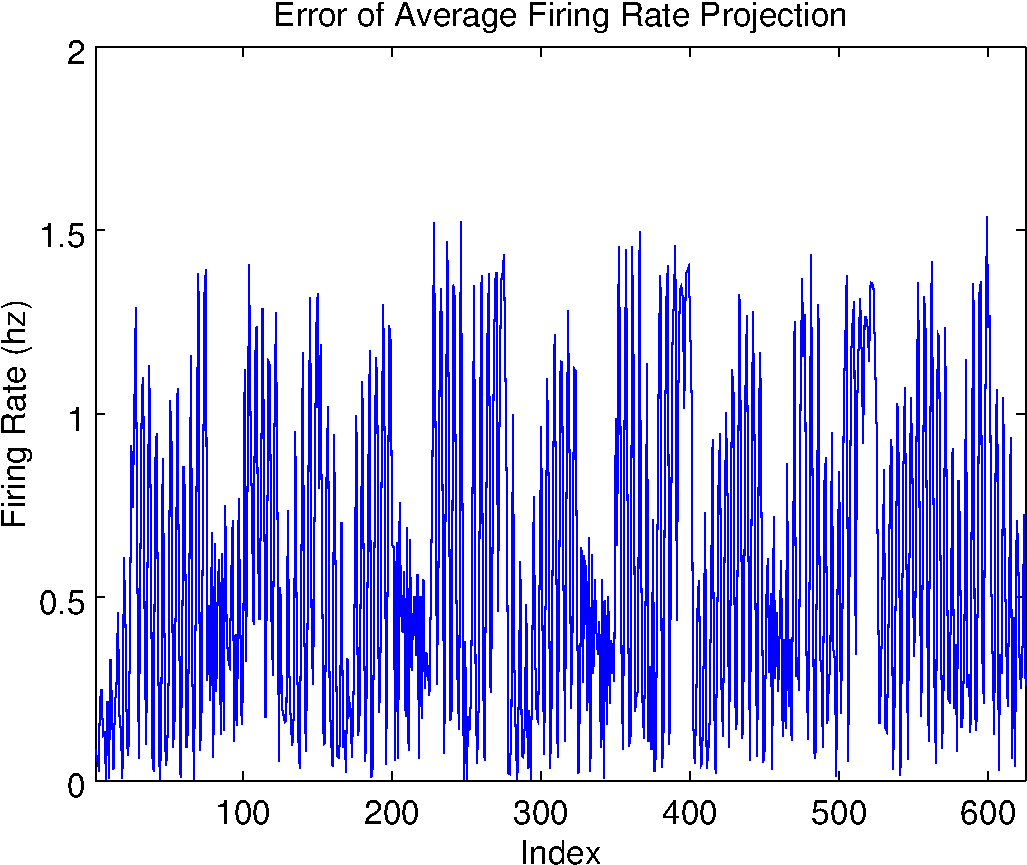
\includegraphics[scale=.5]{AverageFiringRateError.pdf}%
%   \end{center}
% \end{frame}

\begin{frame}\frametitle{Coefficients of Projection}
  \begin{table}
\centering
\resizebox{\linewidth}{!}{%
\begin{tabular}{|c|c|c|c|c|c|}
\hline
 & Constant & F1 & F2 & F3 & F4 \\
\hline
Burst Duration & 96.778146 & -1.594133 & 7.475547 & -0.935241 & -3.481930 \\
\hline
Burst Frequency & 1.265639 & 0.030140 & 0.006260 & 0.131930 & 0.002809 \\
\hline
Spikes Per Burst & 5.897340 & -0.161142 & 0.602120 & -0.089834 & -0.181207 \\
\hline
MMP & -54.414978 & 0.910534 & -0.370228 & -0.034746 & -0.598222 \\
\hline
AMP & -46.512639 & 0.411004 & 0.311948 & 0.180725 & -0.346202 \\
\hline
Peak Firing Rate & 89.765620 & -0.957476 & 2.870573 & -0.255760 & 0.285066 \\
\hline
Average Firing Rate & 62.308708 & -0.834583 & 2.597794 & -0.486379 & 0.076373 \\
\hline
\end{tabular}}
\caption{Coefficients of Projection}
\end{table}
\end{frame}

\begin{frame}\frametitle{Proportions}
  \begin{table}
\centering
\resizebox{\linewidth}{!}{%
\begin{tabular}{|c|c|c|c|c|}
\hline
 & H & CaT & NaP & BK \\
\hline
Burst Duration & 0.1182 & 0.5543 & 0.0693 & 0.2582 \\
\hline
Burst Frequency & 0.1761 & 0.0366 & 0.7709 & 0.0164 \\
\hline
Spikes Per Burst & 0.1558 & 0.5822 & 0.0869 & 0.1752 \\
\hline
MMP & 0.4758 & 0.1935 & 0.0182 & 0.3126 \\
\hline
AMP & 0.3288 & 0.2496 & 0.1446 & 0.2770 \\
\hline
Peak Firing Rate & 0.2192 & 0.6571 & 0.0585 & 0.0652 \\
\hline
Average Firing Rate & 0.2089 & 0.6502 & 0.1217 & 0.0191 \\
\hline
\end{tabular}}
\caption{Proportion of output metrics explained by each signal}
\end{table}
\end{frame}

\begin{frame}\frametitle{Proportions}
  \begin{table}
\centering
\resizebox{\linewidth}{!}{%
\begin{tabular}{|c|c|c|c|c|}
\hline
 & H & CaT & NaP & BK \\
\hline
Burst Duration & 0.1182 & \hl{0.5543} & 0.0693 & \hl{0.2582} \\
\hline
Burst Frequency & 0.1761 & 0.0366 & \hl{0.7709} & 0.0164 \\
\hline
Spikes Per Burst & 0.1558 & \hl{0.5822} & 0.0869 & 0.1752 \\
\hline
MMP & \hl{0.4758} & 0.1935 & 0.0182 & \hl{0.3126} \\
\hline
AMP & \hl{0.3288} & \hl{0.2496} & 0.1446 & \hl{0.2770} \\
\hline
Peak Firing Rate & \hl{0.2192} & \hl{0.6571} & 0.0585 & 0.0652 \\
\hline
Average Firing Rate & \hl{0.2089} & \hl{0.6502} & 0.1217 & 0.0191 \\
\hline
\end{tabular}}
\caption{Proportion of output metrics explained by each signal}
\end{table}
\end{frame}

\begin{frame}\frametitle{Burst Duration}
  \begin{center}
    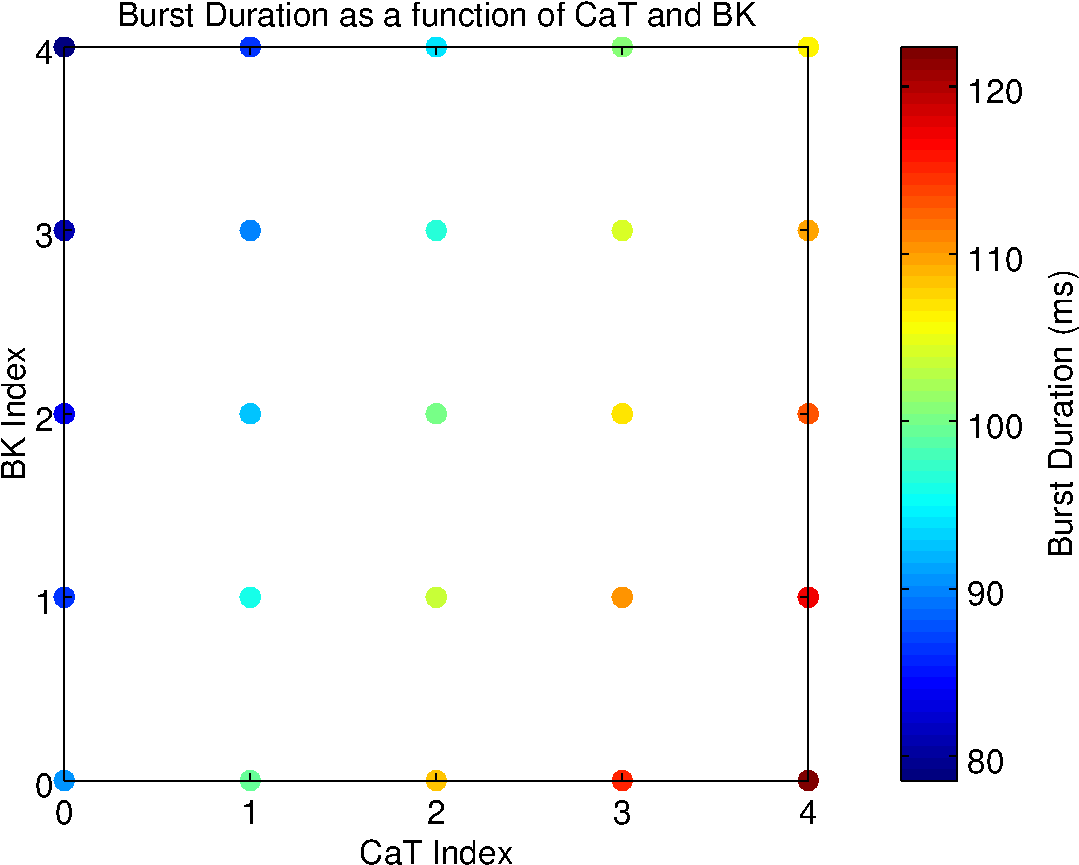
\includegraphics[scale=.5]{BurstDurationScatter.pdf}%
  \end{center}
\end{frame}

\begin{frame}\frametitle{Burst Frequency}
  \begin{center}
    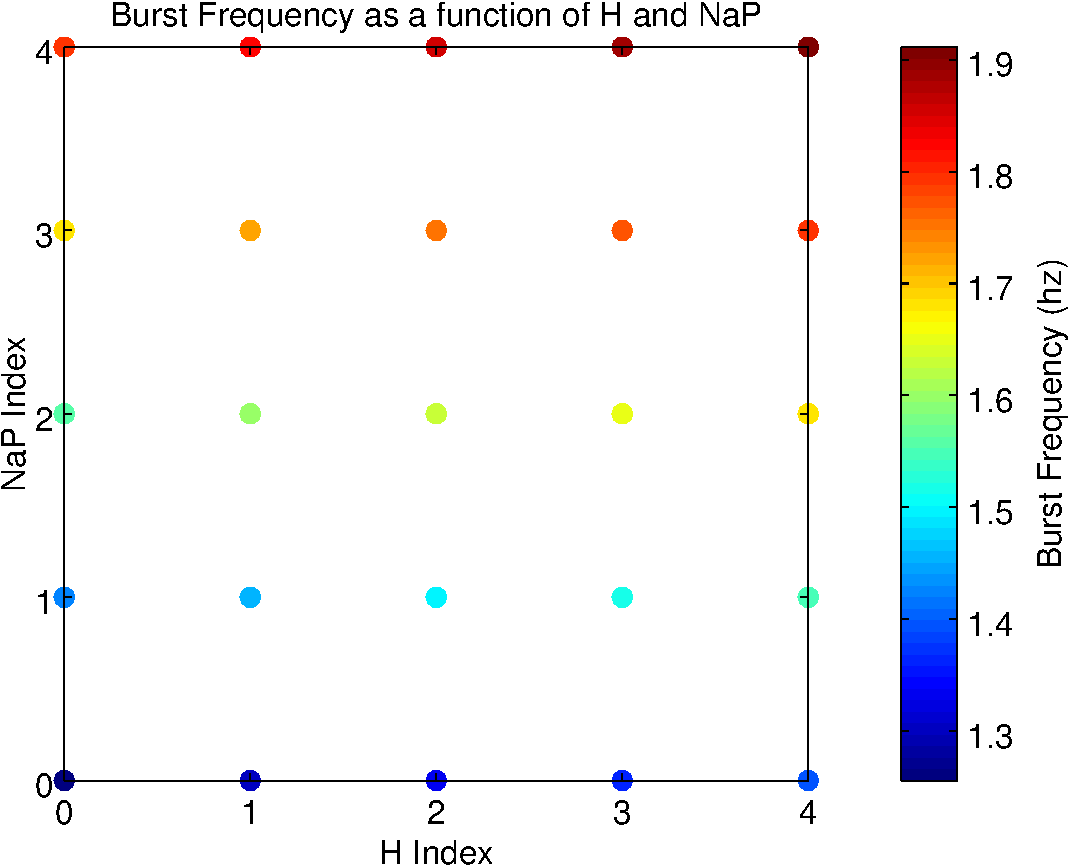
\includegraphics[scale=.5]{BurstFrequencyScatter.pdf}%
  \end{center}
\end{frame}

\begin{frame}\frametitle{MMP}
  \begin{center}
    \includegraphics[scale=.7]{MMPScatter.pdf}%
  \end{center}
\end{frame}

\begin{frame}\frametitle{Variance}
  Projecting variance traces onto the space spanned by $1,F_1,...,F_4$ did not work nicely.
  \begin{center}
    \includegraphics[scale=.32]{BurstDurationVariance.pdf}%
    \includegraphics[scale=.32]{BurstDurationVarianceProjection.pdf}%
  \end{center}
\end{frame}

\begin{frame}\frametitle{Are there any elements that should be avoided?}
  \begin{itemize}
    \item We are not so much concerned with how the parameters shape the variance, but rather simply if there are any sections of parameter space that are too ``sensitive'' and should be avoided
    \item Variance for every metric but burst duration was small, and all mean values fell well within the range of experimentally observed values.
    \item Why is burst duration so sensitive?
  \end{itemize}
\end{frame}

\begin{frame}\frametitle{Burst Duration Sensitivity}
  Element 422 had a high value for variance
  \begin{center}
    \includegraphics[scale=.45]{Element422.pdf}%
  \end{center}
\end{frame}

\begin{frame}\frametitle{Single Bursts}
  Projection method revealed that most of the variability was due to CaT. Holding other parameter values constant and varying CaT from 13.5 to 14 results in a small perturbation of the burst envelope.
  \begin{center}
    \includegraphics[scale=.32]{SingleBurst13p5.pdf}%
    \includegraphics[scale=.32]{SingleBurst14.pdf}%
  \end{center}
\end{frame}

\begin{frame}\frametitle{Overlay}
  \begin{center}
    \includegraphics[scale=.5]{SingleBurstOverlay.pdf}%
  \end{center}
\end{frame}

\section{Discussion}

\begin{frame}\frametitle{Project Discussion}
  Goals of the project proposal were met.\\
  \vspace{1em}
  Project outcomes:
  \begin{itemize}
    \item ME-PCM was implemented efficiently in parallel
    \item Computation on CHPC clusters allowed for more data than possible on workstation
    \item ET-Cell model determined to be insensitive to relative strengths of current Conductances
    \item New conclusions were drawn about the effect of each parameter on output metrics
    \item Developed (novel?) method to analyze the high dimensional output data of the ME-PCM method
  \end{itemize}
\end{frame}

\begin{frame}\frametitle{ME-PCM Discussion}
 \begin{itemize}
   \item The ME-PCM is very general and easy to implement
   \begin{itemize}
     \item User-defined metrics
     \item Metrics need not be continuous functions
     \item Metrics can vary over time (not seen in this presentation)
   \end{itemize}
   \item ME-PCM can be used to quantify system sensitivity and elucidate the effects of parameters on system output
   \item In the limit as the element size goes to zero, the variance within an element converges to the magnitude of the square of the gradient
   \item Claim that multiple metrics can be examined after sampling step was not feasible in practice.
   \item Despite the claimed efficiency improvement over Monte-Carlo methods, any method that requires sampling will not scale well with dimensionality
 \end{itemize}
\end{frame}

\begin{frame}\frametitle{References}
  \printbibliography
\end{frame}

\end{document}
